%%
%% This is file `mcmthesis-demo.tex',
%% generated with the docstrip utility.
%%
%% The original source files were:
%%
%% mcmthesis.dtx  (with options: `demo')
%%
%% -----------------------------------
%%
%% This is a generated file.
%%
%% Copyright (C)
%%     2010 -- 2015 by Zhaoli Wang
%%     2014 -- 2016 by Liam Huang
%%
%% This work may be distributed and/or modified under the
%% conditions of the LaTeX Project Public License, either version 1.3
%% of this license or (at your option) any later version.
%% The latest version of this license is in
%%   http://www.latex-project.org/lppl.txt
%% and version 1.3 or later is part of all distributions of LaTeX
%% version 2005/12/01 or later.
%%
%% This work has the LPPL maintenance status `maintained'.
%%
%% The Current Maintainer of this work is Liam Huang.
%%

\documentclass{mcmthesis}
\mcmsetup{
CTeX = false,
tcn = 72985,
problem = D,
sheet = true,
titleinsheet = true,
keywordsinsheet = true,
titlepage = true
}

\usepackage{palatino}
\usepackage{mwe}
\usepackage{graphicx}
\usepackage{subcaption}
\usepackage{float}
\usepackage{multirow}
\usepackage{indentfirst}
\usepackage{gensymb}
\usepackage[ruled,vlined,commentsnumbered]{algorithm2e}
\usepackage{geometry}
%\usepackage{subfigure}
%\geometry{left=2cm,right=2cm,top=2cm,bottom=2cm} %%页边距

\newtheorem{myassump}{Assumption}
\newtheorem*{myreason}{Reason}

\begin{document}
\linespread{1} %%行间距
\setlength{\parskip}{0.5\baselineskip} %%段间距
\title{CNEM: An Effective and Adaptive Model for Charging Network Evolution}
\date{}

\begin{abstract}
Recent years have witnessed a growing tendency to adopt electric vehicles (EVs). To achieve a migration towards full EV system, it is urgent for countries to work out a plan for charging network evolution.

In order to help countries develop policies for evolving charging network, we propose an effective and adaptive model CNEM (Charging Network Evolution Model). CNEM is composed of three submodels, Charging Station Location Model (CSLM), Iterative Evolution Model for Charging Network (CN-IEM), and Classification Model (CM).

CSLM is used to determine the locations of charging stations in the final charging network. In CSLM, we make a combination between \textbf{node-covering model} and \textbf{flow-capturing model}, and use \textbf{Fuzzy C-Means} (FCM) clustering algorithm to determine the locations of charging stations.

CN-IEM is used to control the process of evolving charging network. In CN-IEM, we use \textbf{iterative evolution model} to simulate the mutual promotion between deployment of charging network and purchase of EV over time.

CM is used to classify different countries and design a plan that works best for a specific country. In CM, we introduce seven classification criteria and present corresponding modification based on the practical condition of a country.

Furthermore, we explain the possible impacts of emerging technologies on charging network evolution. Sensitivity analysis is carried out, and the strength and weakness of our models are also discussed.

We apply CSLM to the United States and obtain the locations of charging stations in the final charging network. Moreover, we apply CN-IEM to South Korea to show the evolving process of charging network. Results prove the effectiveness of our models.
\begin{keywords}
Charging Network; Fuzzy C-Means Clustering; Iterative Evolution; Traffic Simulation
\end{keywords}
\end{abstract}

\maketitle

\tableofcontents

\newpage

\section{Introduction}
\subsection{Background}\label{Sec-Background}
Due to the global interest to reduce the use of fossil fuels, many countries are starting to adopt electric vehicles (EVs). To migrate successfully to a full EV system, governors are in need of effective plans for evolving charging network.

Some works have been devoted to charging station location problem. There are mainly two types of model: node-covering and flow-capturing. \cite{Xi2013} combines simulation with optimization model to meet the charging demand in some city areas like retail store, university, and supermarket. \cite{Shi2014} uses clustering method to find out the best charging locations. \cite{Dong2016} find candidate locations with high demand density by simulation and uses the share nearest neighbour clustering to select the best locations of charging stations. \cite{Kim2012} tries to locate the refueling places vehicles can access with the shortest deviation from their original route. \cite{Wu2017} uses stochastic programming to study the flow capturing location problem under uncertainty.

In practice, several business companies have achieved desirable results. One of them is Tesla. Tesla has received a large number of reservations of Tesla Model 3, a class of Tesla cars with affordable price, from all over the world. Additionally, Tesla's charging networks have taken shape in Asia, North America, Europe, and Middle East, and the scale of them is growing rapidly. Fig.~\ref{Fig-TeslaStationDistribution} shows the distribution of Tesla supercharger stations in North America.

\begin{figure}[htbp]
  \centering
  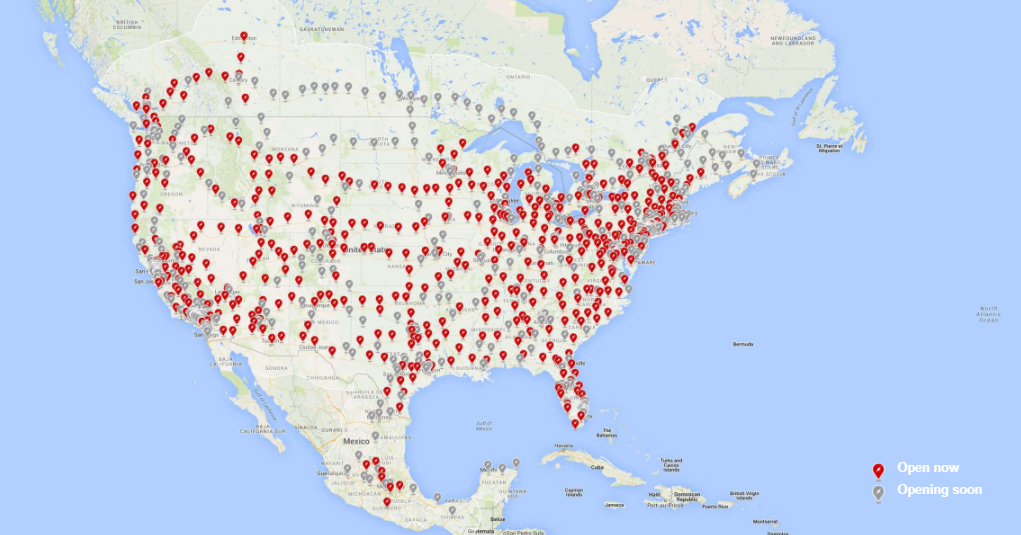
\includegraphics[width=0.8\textwidth]{TeslaStationDistribution.PNG}
  \caption{Distribution of Tesla Supercharger Stations in North America~\cite{Supercharging}}\label{Fig-TeslaStationDistribution}
\end{figure}

With the development of technology, EV adoption is put on agenda by many countries. The primary aspect that should be taken into consideration is the final architecture of the charging network. Since each country has its own specific conditions, it is urgent to design a model with high adaptability. Moreover, evolution model is required to help control the timeline for evolving charging network.
\subsection{Overview of Our Work}
In this paper, we propose CNEM, a model composed of Charging Station Location Model (CSLM), Iterative Evolution Model for Charging Network (CN-IEM), and Classification Model (CM). CSLM combines node-covering model with flow-capturing model and uses Fuzzy C-Means (FCM) clustering algorithm to obtain best locations. CN-IEM simulates the mutual promotion between the deployment of charging stations and the purchase of EV with an iterative evolution model. In CM, we set seven classification criteria and present corresponding modification to adapt our model to different countries. We explain how emerging technologies impact on the charging network. We also make sensitivity analysis and present the strength and weakness of our models. Experiments of CSLM and CN-IEM are conducted for United States and South Korea respectively. Results prove the effectiveness of our models.

We arrange the rest of this paper in the following way. Section~\ref{Sec-Nomenclature} lists the nomenclature used in our paper. In Section~\ref{Sec-Task1}, we propose CSLM and give solution to Task 1. In Section~\ref{Sec-Task2}, we propose CN-IEM and give solution to Task 2. In Section~\ref{Sec-Task3}, we propose CM and introduce the corresponding modification. In Section~\ref{Sec-Task4}, we discuss the possible impacts of emerging technologies on charging network. Sensitivity Analysis and strength and weakness are presented in Section~\ref{Sec-Analysis}. Finally, we make some conclusions in Section~\ref{Sec-Conclusion}.
\section{Nomenclature}\label{Sec-Nomenclature}
Main symbols used in this paper are listed in Table~\ref{Tbl-Nomenclature}. Details of these symbols are explained in the rest of the paper.

\begin{table}[htbp]
  \centering
  \caption{List of Nomenclature}\label{Tbl-Nomenclature}
  \begin{tabular}{ll}
    \toprule
    Symbol & Definition \\
    \midrule
    $c_{i}$ & the $i^{th}$ cluster in a state \\
    $cs_{i}$ & the charging station constructed at the center of $c_{i}$ \\
    $n_{ev}^{c_{i}}$ & number of EVs in $c_{i}$ \\
    $n_{ch}^{cs_{i}}$ & number of chargers in $cs_{o}$ \\
    $\alpha$ & possibility of meeting the need of charging \\
    $ev_{i}$ & the $i^{th}$ EV in simulation \\
    $soc_{i}^{full}$ & full state of charge of $ev_{i}$ \\
    $soc_{i}^{thre}$ & threshold state of charge of $ev_{i}$ \\
    $\tau$ & tolerance of the user of $ev_{i}$ \\
    $w$ & electricity consumed for a unit distance \\
    $s$ & distance passed after last charging \\
    $den_{ev}^{(i)}$ & density of EVs in the $i^{th}$ iteration \\
    $den_{cs}^{(i)}$ & density of charging stations in the $i^{th}$ iteration \\
    $state_{i}$ & the $i^{th}$ state of a country \\
    $n_{ev}^{state_{i}}$ & number of EVs in $state_{i}$ \\
    $n_{ev}^{thre}$ & threshold for the number of EVs in a state \\
    $n_{cand}^{state_{i}}$ & number of candidate sites in $state_{i}$ \\
    \bottomrule
  \end{tabular}
\end{table}
\section{Task 1: Charging Station Location Model (CSLM)}\label{Sec-Task1}
\subsection{Model Selection}
As mentioned in Section \ref{Sec-Background}, there are mainly two types of models addressing the location problem. One is node-covering model, which determines the locations of charging stations according to factors, such as the density of electric vehicles and the density of population. The other is flow-capturing model, in which road traffic flow is the main aspect considered.

These two types of models complement each other. For areas with high EV density or high population density, charging stations obtained from flow-capturing model are usually not enough, while node-covering model also results in insufficient charging stations in sparsely populated regions along important long-distance roads.

Based on the characteristics of them, we make a combination of both models. We consider the locations of charging stations from two aspects: intrastate and interstate. Within a state, EVs are relatively concentrated, so we apply node-covering model to find out the locations of destination charging stations~\cite{DestinationCharging}. Between states, supercharging stations~\cite{Supercharging} should be constructed mainly along interstate highways, so we use the flow-capturing model.
\subsection{Assumptions}
\begin{myassump}\label{Assump-TAZ}
The number of vehicles in each traffic analysis zone (TAZ) is the same.
\end{myassump}
\noindent\textbf{Reason:} The level of traffic activity of each TAZ is similar, and there is be a positive correlation between traffic activity and the number of vehicles.

\begin{myassump}\label{Assump-Poisson}
The number of electric vehicles arriving at a charging station within the average charging time in a certain region follows Poisson Process.
\end{myassump}
\noindent\textbf{Reason:} Poisson Process is commonly used to illustrate the number of random events within a time unit. We use Poisson Process to simulate the number of EVs in need of charging.

\begin{myassump}\label{Assump-FullSOC}
Full state of charge of an EV follows Uniform Distribution.
\end{myassump}
\noindent\textbf{Reason:} Because of battery aging, full state of charge of a battery cannot reach 100\% and may decrease to a certain range. We use uniform distribution to describe the value of full state of charge in this range.

\begin{myassump}\label{Assump-Tolerance}
Tolerance follows Uniform Distribution.
\end{myassump}
\noindent\textbf{Reason:} When the electricity of an EV drops to a certain level, the user will search for charging stations to get the EV charged. Some people is prudent, searching for charging stations when there is still much electricity, while some people can tolerate the a very low-level state of charge. We use uniform distribution to describe the value of tolerance in a certain range.

\begin{myassump}\label{Assump-Simulation}
In the simulation in Section~\ref{Sec-Interstate}, an EV immediately gets charged to full state of charge when it reaches a charging point.
\end{myassump}
\noindent\textbf{Reason:} In order to use charging points for location determination, we make EVs get charged in place and continue to head for their destinations. Since charging points are concentrated and the distance between a charging point and the actual charging station is short, this simplification has little influence to the final result.
\subsection{Intrastate CSLM}\label{Sec-Intrastate}
We consider a state to the level of traffic analysis zone (TAZ)~\cite{TrafficAnalysisZone}. A TAZ is a basic geographic unit usually used in transportation planning. According to \cite{TrafficAnalysisZone}, a common method for simplification is ``to collapse each zone to a single point''. We use geometric center to represent a TAZ, and then a state can be represented by a set of points. According to Assumption~\ref{Assump-TAZ}, since we only consider personal passenger vehicles, these points actually reflect the distribution of EVs. Intuitively, the more concentrated the distribution of EVs is, the higher the demand for charging stations should be. In other words, charging station locations should be consistent with the distribution of EVs.

We modify the methods in \cite{Shi2014} and apply fuzzy C-Means (FCM) clustering algorithm to the set of points in a state. FCM is a clustering algorithm which allows a data point to belong to two or more clusters. This property is consistent real life, in which an EV may go to one of the nearby charging stations but not certainly the nearest one. After clustering, we obtain a set of clusters $C=\{c_{1},c_{2},\cdots\}$. A destination charging station $cs_{i}$ is constructed at the center of cluster $c_{i}$.

Then we determine the number of chargers in a charging station. According to Assumption~\ref{Assump-Poisson}, the number of EVs arriving a charging station within the average charging time in a certain cluster $c_{i}$ follows Poisson Process, where $\lambda$ is the average number of EVs arriving this charging station within a time unit in $c_{i}$. We denote the number of EVs in $c_{i}$ as $n_{ev}^{c_{i}}$ and the number of chargers in $cs_{i}$ as $n_{ch}^{cs_{i}}$. $\lambda$ is proportional to $n_{ev}^{c_{i}}$. The number of EVs in need of charging within the average charging time in $c_{i}$ follows the distribution in Eqn.~\eqref{Eqn-Poisson}.

\begin{equation}\label{Eqn-Poisson}
P\left[N(t+t_{0})-N(t)=k\right]=e^{-\lambda t_{0}}\dfrac{(\lambda t_{0})^{k}}{k!},\quad\lambda\propto n_{ev}^{c_{i}},\quad k=0,1,\cdots
\end{equation}

We hope the charging station can meet the need of charging with a possibility not lower than $\alpha$, as shown in Eqn.~\eqref{Eqn-ChargerNumber}.

\begin{equation}\label{Eqn-ChargerNumber}
\begin{split}
P\left[N(t+t_{0})-N(t)\leq n_{ch}^{cs_{i}}\right] & =\sum_{i=0}^{n_{ch}^{cs_{i}}}\dfrac{(\lambda t_{0})^{i}}{i!}e^{-\lambda t_{0}} \\
  & =e^{-\lambda t_{0}}\sum_{i=0}^{n_{ch}^{cs_{i}}}\dfrac{(\lambda t_{0})^{i}}{i!}\geq\alpha
\end{split}
\end{equation}
Setting an $\alpha$, the minimum number of chargers in a charging station can be determined by solving Eqn.~\eqref{Eqn-ChargerNumber}.
\subsection{Interstate CSLM}\label{Sec-Interstate}
We use an undirected graph to represent the traffic between states, in which each state is a point and interstate highways are edges. In this graph, similar to~\cite{Dong2016}, we simulate the travelling actions of EVs to determine the locations of supercharging stations.

We first initialize a set of EVs denoted as $EV=\{ev_{1},ev_{2},\cdots\}$. A uniformly random origin-destination pair (O-D pair) is allocated to each EV, indicating its starting point and terminal point. Each EV is also assigned with its full state of charge and its threshold state of charge, denoted as $soc_{i}^{full}$ and $soc_{i}^{thre}$. Full state of charge means the maximum state of charge each time an EV get charged, and an EV should search for charging stations when its state of charge drops to threshold state of charge. According to Assumption~\ref{Assump-FullSOC}, $soc_{i}^{full}$ follows uniform distribution $U(soc_{l},soc_{u})$. $soc_{i}^{thre}$ is defined as $soc_{i}^{thre}=\tau soc_{i}^{full}$, where $\tau$ is the tolerance which also follows uniform distribution $U(\tau_{l},\tau_{u})$ according to Assumption~\ref{Assump-Tolerance}. We define the state of charge of $ev_{i}$ in Eqn.~\eqref{Eqn-StateOfCharge}, where $w$ is the electricity consumed for a unit distance and $s$ is the distance passed after last charging.

\begin{equation}\label{Eqn-StateOfCharge}
soc_{i}=soc_{i}^{full}-ws
\end{equation}

During simulation, each EV leaves its origin and heads for its destination through interstate highways. All along the road, the electricity is gradually consumed and finally drops to threshold state of charge. We call the point where electricity drops to threshold state of charge charging point. According to Assumption~\ref{Assump-Simulation}, we suppose an EV gets charged to full state of charge upon reaching a charging point. Then the EV continue to head for its destination. An EV may reach several charging points before it arrives at its destination. All the EVs travel in the same way. Fig.~\ref{Fig-ChargingPointExample} shows the trip of an EV. It starts with full state of charge. Electricity drops to threshold at the first charging point, and it get charged to full state of charge immediately. The whole trip contains two charging points.

\begin{figure}[htbp]
  \centering
  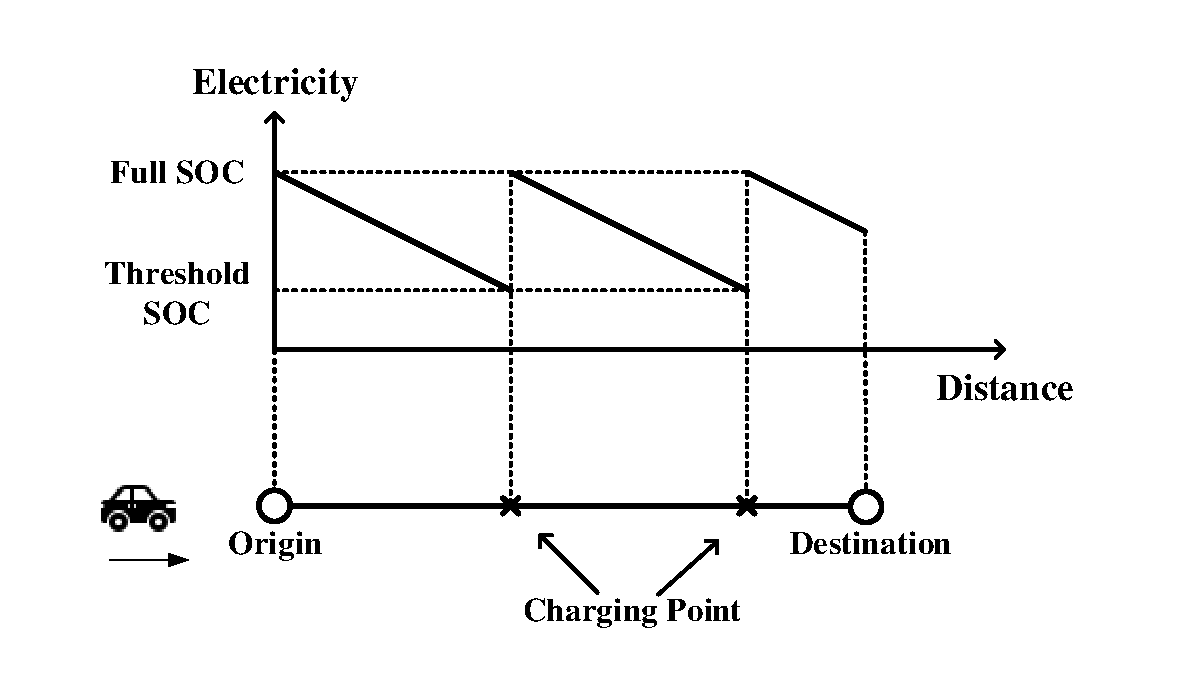
\includegraphics[width=0.8\textwidth]{ChargingPoint.pdf}
  \caption{Trip of an EV Containing Two Charging Points}\label{Fig-ChargingPointExample}
\end{figure}

After simulation, we obtain a large number of charging points distributed along the highways. We still apply Fuzzy C-Means (FCM) clustering algorithm to these points and construct a supercharging station at the center of each cluster. Then we determine the number of chargers in each charging station using the same method as in Section~\ref{Sec-Intrastate}.
\subsection{Model Solution}
We apply Charging Station Location Model (CSLM) to the United States and obtain the locations of charging stations when everyone switches to all-electric passenger vehicles. By comparing the current locations of Tesla charging stations and the final locations obtained from our model, we make an evaluation of Tesla's location selection.

We apply Intrastate CSLM to the 51 states in the United States. States are divided to the level of traffic analysis zone (TAZ), and each TAZ is represented by its geometric center. Fig.~\ref{Fig-USTAZ} shows the distribution of TAZ in the United States, and Fig.~\ref{Fig-CATAZ} shows the distribution in California as an example.

\begin{figure}[H]
    \centering
    \begin{subfigure}[b]{0.45\textwidth}
		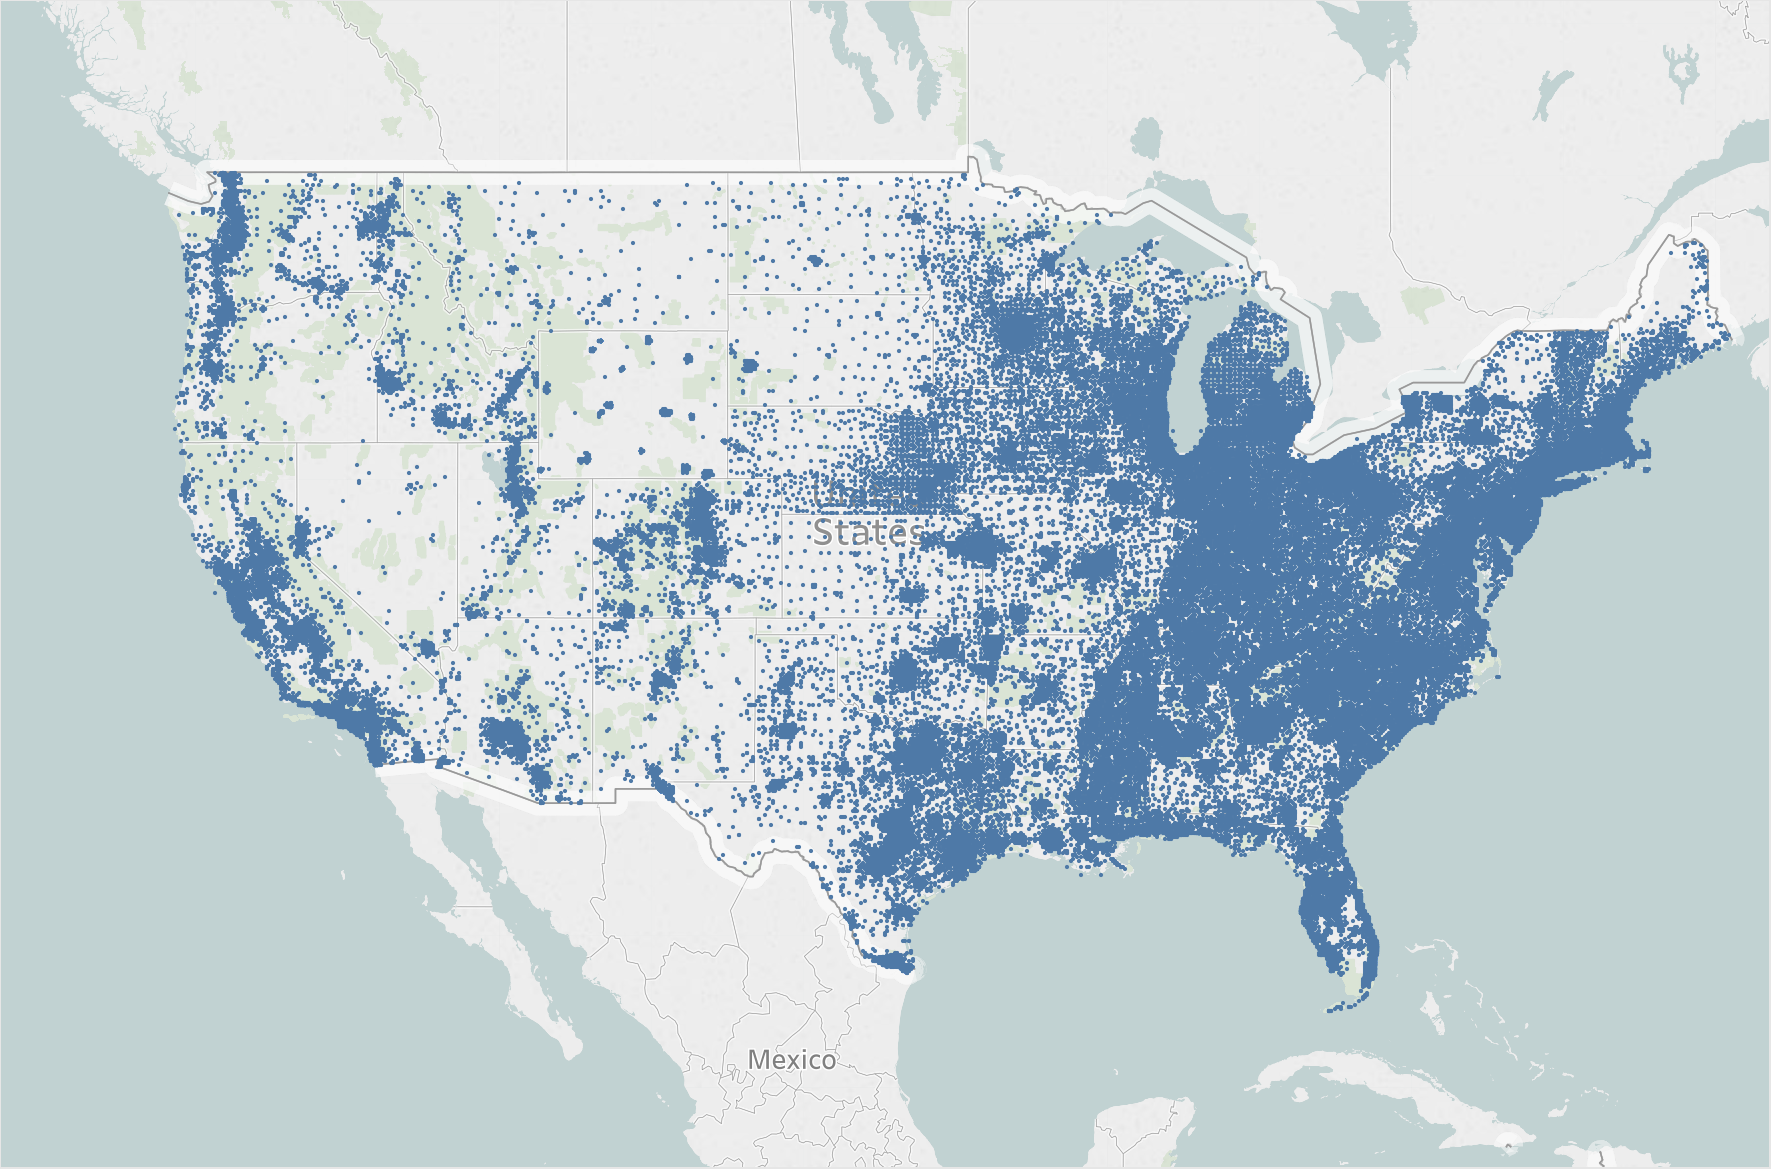
\includegraphics[width=0.95\textwidth]{USTAZ.png}
		\caption{United States}
		\label{Fig-USTAZ}
	\end{subfigure}
    \begin{subfigure}[b]{0.45\textwidth}
		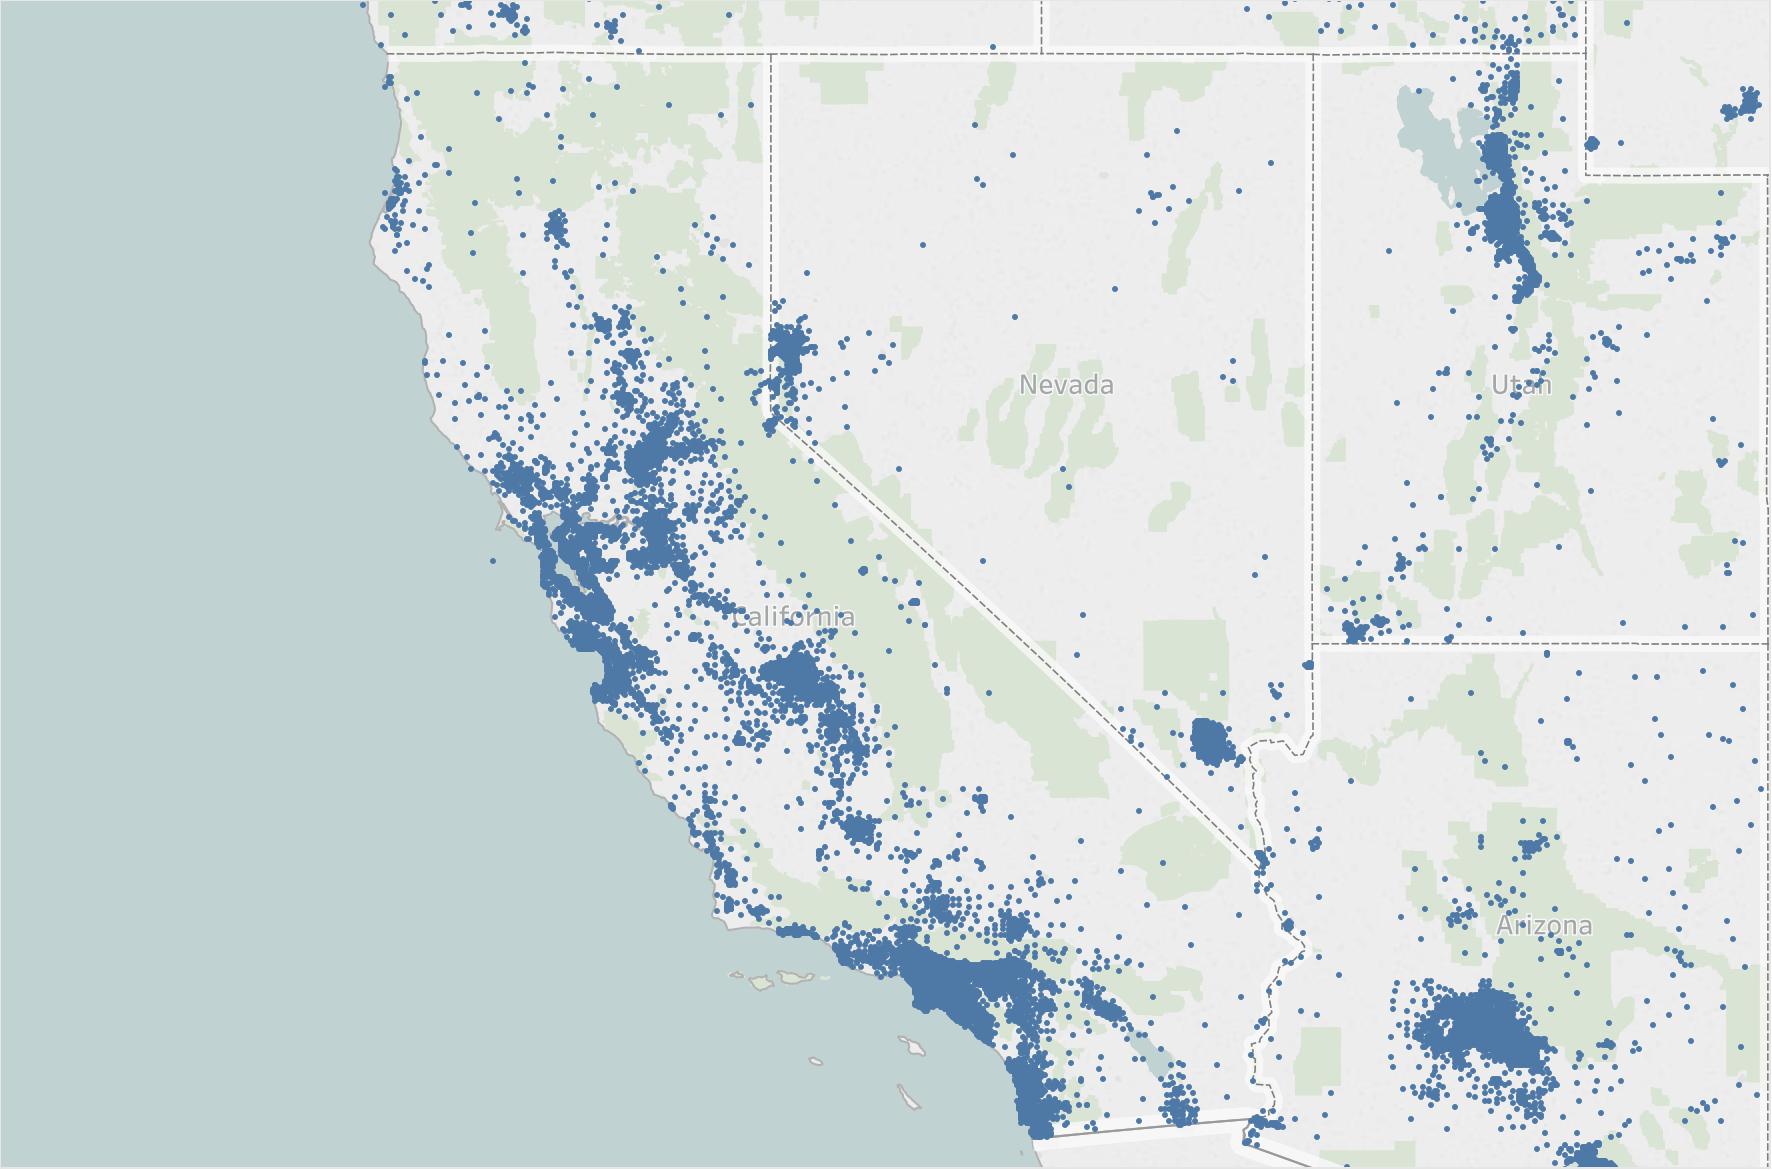
\includegraphics[width=0.95\textwidth]{CATAZ.png}
		\caption{California}
		\label{Fig-CATAZ}
	\end{subfigure}
    \caption{TAZ Distribution}
\end{figure}

Fuzzy C-Means (FCM) algorithm is used for clustering. We obtain 5604 clusters in all. At each of these centers, a destination charging station should be constructed.

Then we apply Interstate CSLM to the whole country. After simulation, we do clustering analysis of charging points using FCM algorithm and obtain 893 clusters. A supercharging station should be constructed at the center of each cluster. Fig.~\ref{Fig-USFinal} shows the distribution of all charging stations, in which blue points represent destination charging station, and orange points represent supercharging stations.

\begin{figure}[htbp]
  \centering
  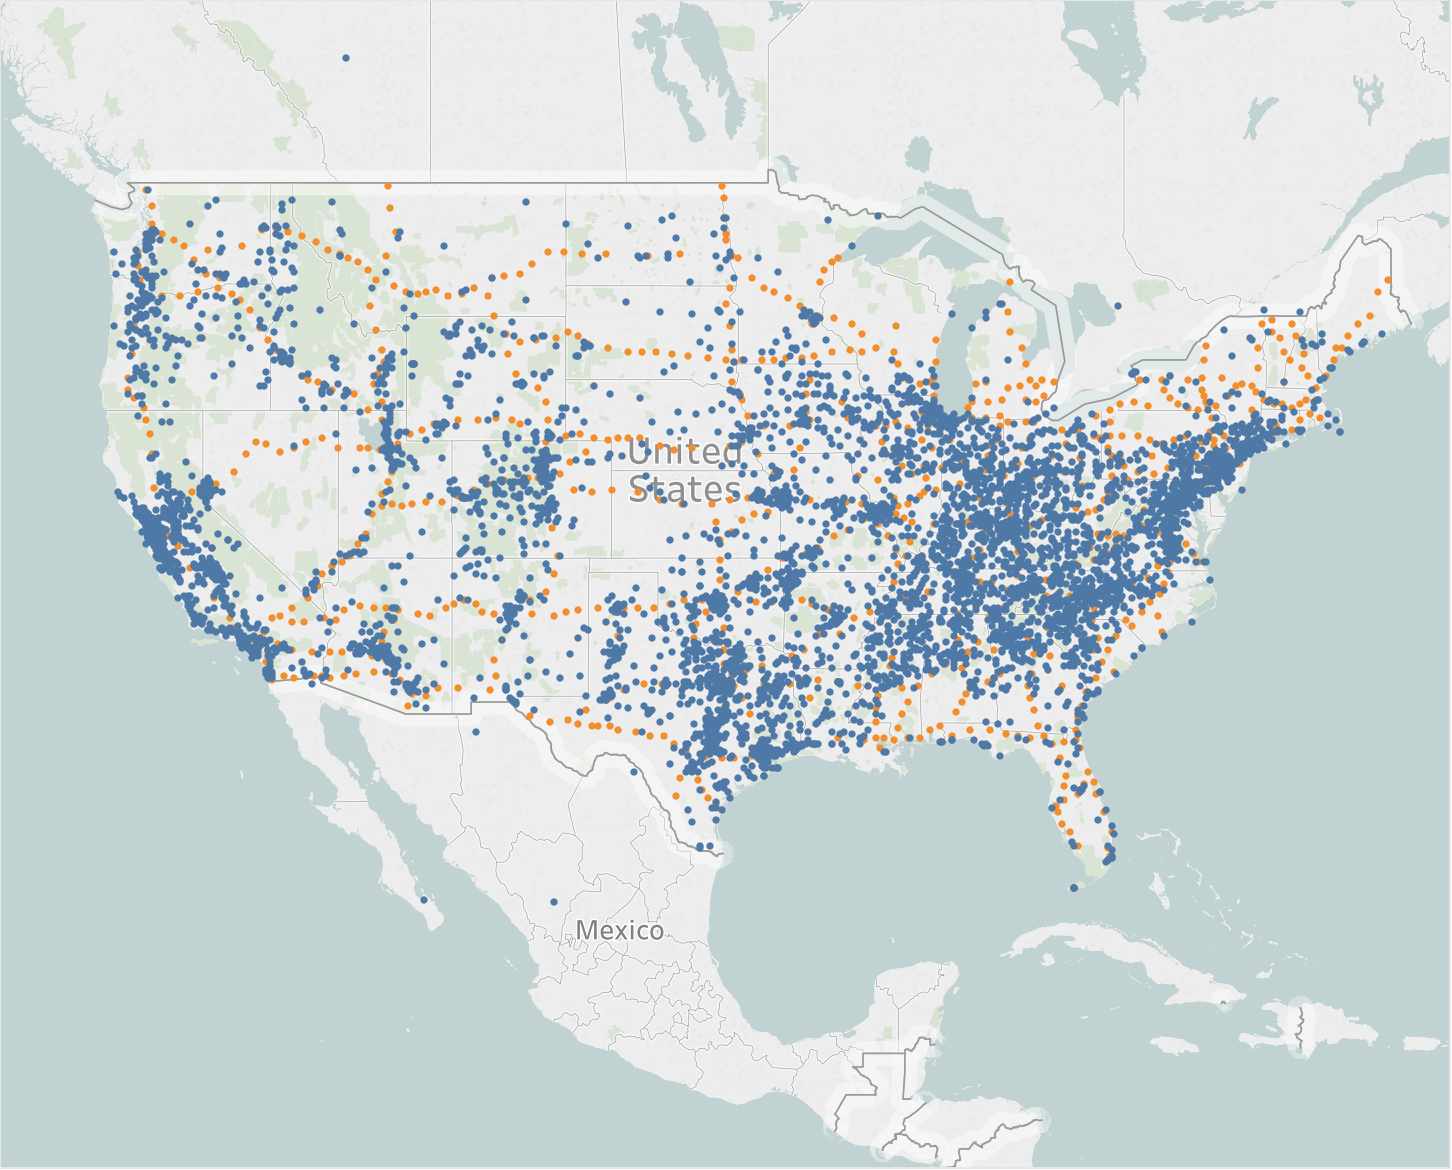
\includegraphics[width=0.6\textwidth]{USFinal.png}
  \caption{Centers of All Clusters in the United States}\label{Fig-USFinal}
\end{figure}

We select same number of charging stations as Tesla by descending order of EV number, as shown in Fig.~\ref{Fig-OurModel2017}. Fig.~\ref{Fig-Tesla2017} shows the current locations of Tesla charging stations. To make a comparison, we match each Tesla charging station with the nearest charging station in our model. The average distance between Tesla charging station and our charging station is 13.510976 km. Based on this statistics, we can judge that location selection of Tesla charging stations is quite reasonable and Tesla is right on the track to a complete switch to all-electric in the United States.

\begin{figure}[htbp]
    \centering
    \begin{subfigure}[b]{0.45\textwidth}
		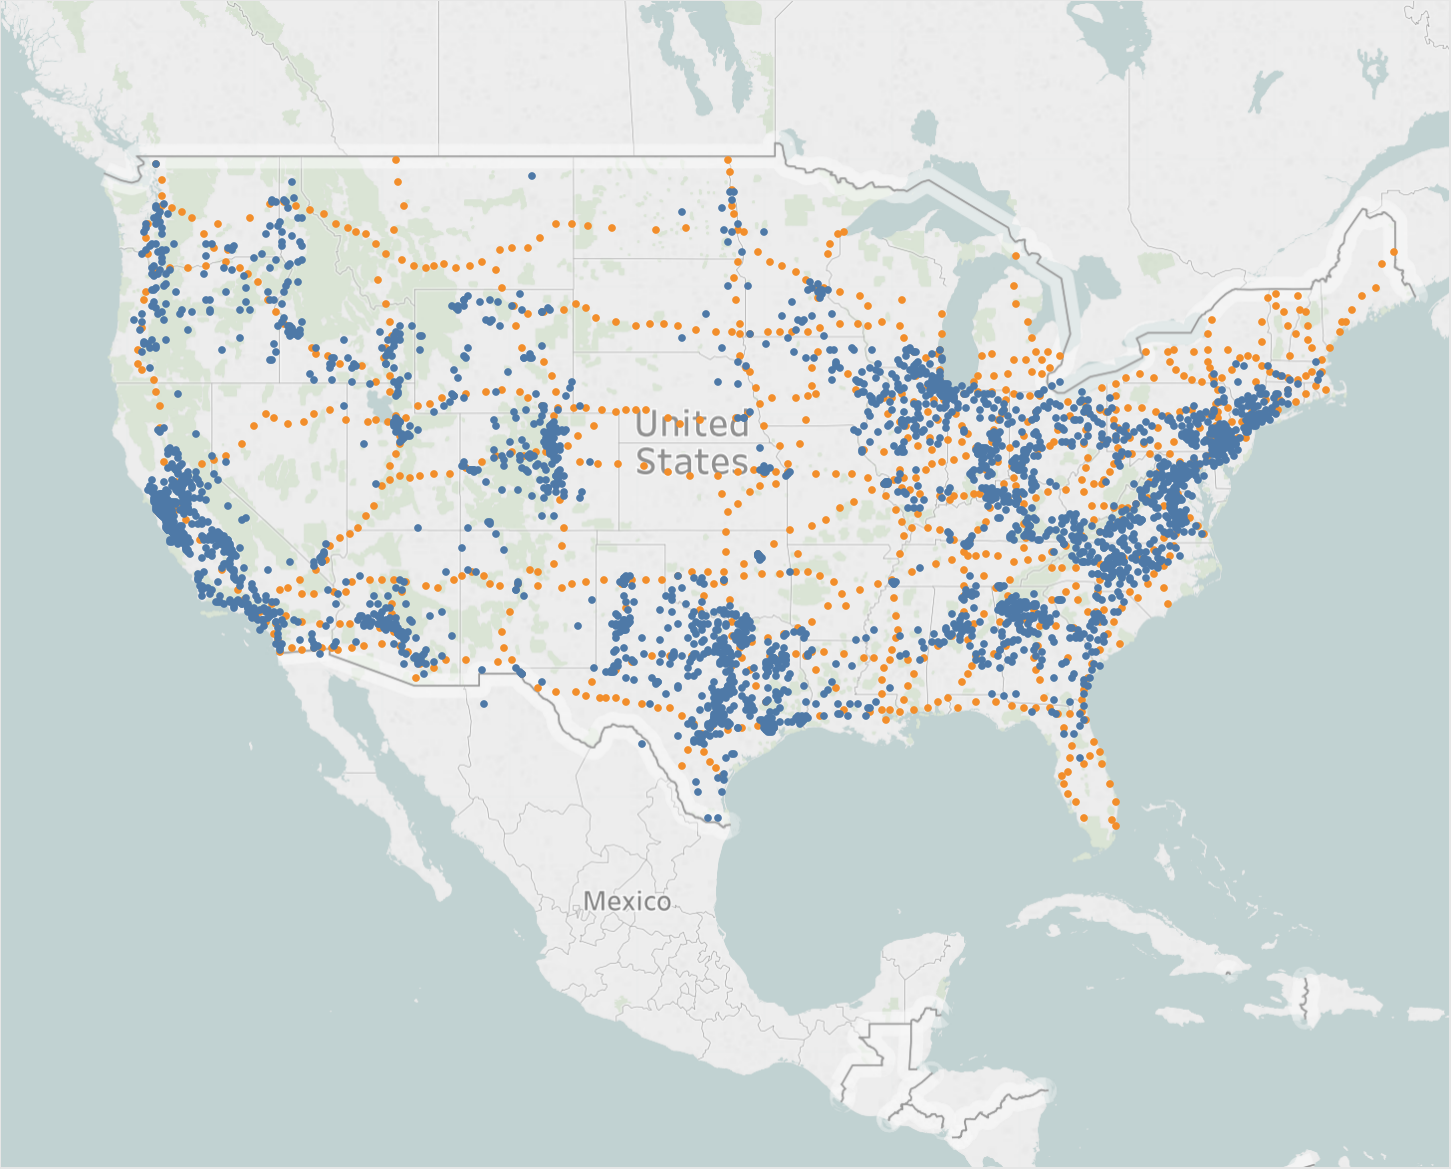
\includegraphics[width=0.95\textwidth]{OurModel2017.png}
		\caption{Our Model}
		\label{Fig-OurModel2017}
	\end{subfigure}
    \begin{subfigure}[b]{0.45\textwidth}
		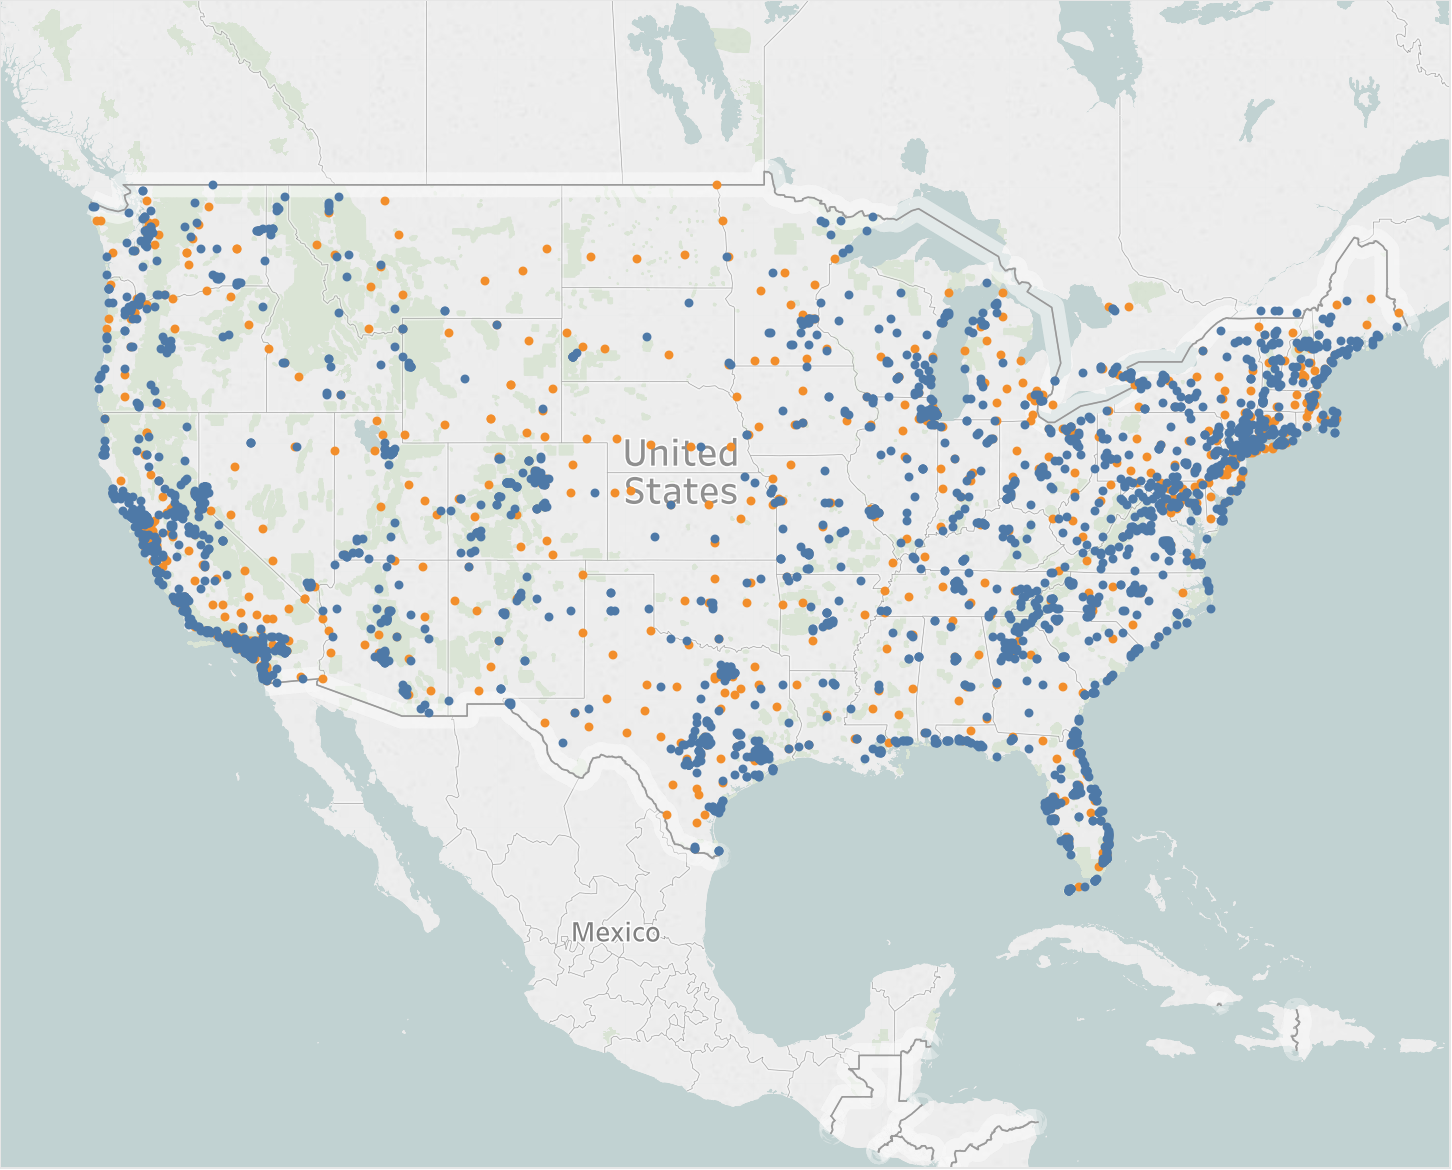
\includegraphics[width=0.95\textwidth]{Tesla2017.png}
		\caption{Tesla}
		\label{Fig-Tesla2017}
	\end{subfigure}
    \caption{Comparison between the Results of Our Model and Tesla's Charging Stations}
\end{figure}

To realize a complete switch to all-electric in the United States, totally 6497 charging stations are in need, including 5604 destination charging stations and 893 supercharging stations. We assume the range 20\% out of urban area is suburban area. Among all the charging stations, 1253 are distributed in urban areas, 1554 are distributed in suburban areas, and 3690 are distributed in rural areas. This indicates that more charging stations are constructed in rural areas than urban areas. However, the density of charging stations in urban areas is much higher than that in rural areas.
\section{Task 2: Iterative Evolution Model for Charging Network (CN-IEM)}\label{Sec-Task2}
\subsection{Ideas of Model}
To establish a model to evolve charging network from zero chargers to full electric-vehicle system, several aspects should be taken into consideration. Firstly, since evolution cannot be realized overnight due to limited budget, phased strategy must be adopted. Secondly, the frequency of daily business is much higher than that of long-distance trips, so the demand for charging stations is higher in urban areas than in suburban and rural areas. Based on this, charging stations should first be constructed in some urban areas and then be deployed simultaneously in the rest of urban areas, suburban areas, and rural areas. Finally, similar to the classic ``chick-and-egg'' question, deployment of charging stations and purchase of electric vehicles are of mutual promotion. As a result, the interaction between them should be considered and charging network evolution should keep pace with the popularity of EV.
\subsection{Assumptions}
\begin{myassump}\label{Assump-EVDensity}
The density of electric vehicles is the same for all cities.
\end{myassump}
\noindent\textbf{Reason:} The density of electric vehicles in a state is influenced specifically by many local factors, but generally by national policy. We ignore the specific factors for simplification.
\subsection{Model Establishment}\label{Sec-IEMEstablishment}
Considering that deployment of charging stations and purchase of electric vehicles promote each other mutually, we build an iterative model to reflect the interaction between them along the timeline. Alg.~\ref{Alg-IterativeEvolution} describes the procedures of this model. Details are explained in the following.

\begin{algorithm}[htbp]
\caption{$Iterative Evolution$}\label{Alg-IterativeEvolution}
$Intrastate-CSLM()$\;
$i=1$\;
$Initialize(den_{ev}^{(i)})$\;
\While{$den_{ev}^{(i)}<1$}{
\ForEach{$state_{i}$}{
\If{$n_{ev}^{state_{i}}\geq n_{ev}^{thre}$}{
Construct destination charging stations in $state_{i}$\;
}
}
\If{$den_{ev}^{i}>den_{ev}^{thre}$}{
Construct supercharging stations along highways\;
}
Calculate $den_{cs}^{(i)}$\;
$den_{ev}^{(i+1)}=Promote(den_{cs}^{(i)})$\;
$i++$\;
}
\Return{$i$}\;
\end{algorithm}

We initially use Intrastate Charging Station Location Model (Intrastate CSLM) in Section~\ref{Sec-Intrastate} to find out all the cluster centers as candidate sites. Initial EV density $den_{ev}^{(1)}$ is related to people's interest, and we assign it with a very small value. $den_{ev}^{(i)}$ is a number in the range of $(0,1)$.

In the first phase, we only construct destination charging stations in states in which the number of EVs reaches a threshold $n_{ev}^{thre}$. The set of states is denoted as $State=\{state_{1},state_{2},\cdots\}$, and the number of EVs in $state_{i}$ is denoted as $n_{ev}^{state_{i}}$, which is the multiplication of EV density and state population. According to Assumption~\ref{Assump-EVDensity}, we suppose EV density is the same for all states. If $n_{ev}^{state_{i}}$ reaches the threshold $n_{ev}^{thre}$, we will begin to construct destination charging stations in $state_{i}$.

In $state_{i}$, suppose there are $n_{cand}^{state_{i}}$ candidate sites. Since EV density is not so high, we do not need to construct charging stations at all candidate sites in a single phase. Therefore, we sort clusters in the descending order of the number of EVs and construct destination charging stations at the centers of top $\lceil den_{ev}n_{cand}^{state_{i}} \rceil$ clusters.

After constructing charging stations in all the states that reach the threshold, we have a new charging station density $den_{cs}^{(1)}$. It can be calculated by the number of charging stations in all states. The increased charging station density encourages people to buy even more EVs. In \cite{Li2017}, impacts of seven factors on EV density is studied using a multiple linear regression model. We make use of its result shown in Eqn.~\eqref{Eqn-EVDenCSDen}, and thus get a new EV density $den_{ev}^{(2)}$ based on $den_{cs}^{(1)}$. The difference in superscript indicates the hysteresis of such impact. Slight changes in all the other factors are ignored.

\begin{equation}\label{Eqn-EVDenCSDen}
\begin{split}
\log(ev-density)= & \beta_{1}(renewables)+\beta_{2}\log(gasprice) \\
  & +\beta_{3}\log(charger-density)+\beta_{4}(education) \\
  & +\beta_{5}\log(population-density)+\beta_{6}\log(pergdp) \\
  & +\beta_{7}(urbanization)+\gamma+\mu+\varepsilon
\end{split}
\end{equation}

In the second phase, we use $den_{ev}^{(2)}$ to construct destination charging stations in states, and then we can obtain $den_{cs}^{(2)}$. Phase by phase, we construct charging stations according to the EV density in the current phase, and the growth of charging station density, in turn, has an impact on the EV density of next phase. Iteratively, charging network develops further and further and finally evolves to full network.

Additionally, when EV density reaches a threshold $den_{ev}^{thre}$, we begin to use Interstate Charging Station Location Model (Interstate CSLM) in Section~\ref{Sec-Interstate} to construct supercharging stations along interstate highways. In each phase, we construct supercharging stations along highways that connect states in which we have already constructed destination charging stations.

Fig.~\ref{Fig-Iteration} illustrates an example of iterative evolution. In Phase 1, no charging station is constructed. In Phase 2, destination charging stations at part of the candidate sites in state $A$ are constructed. In Phase $i$, state $B$ is completely constructed, and state $B$ and $C$ are partially constructed. In this phase, EV density reaches the threshold, so we begin to construct supercharging stations along highways. Since state $A$, $B$, and $C$ have been constructed, supercharging stations are constructed along highways connecting these states. In Phase $i+1$, state $D$ also get partially constructed, so the rest highways are constructed. Finally, all the states and highways are completely constructed.

\begin{figure}[htbp]
  \centering
  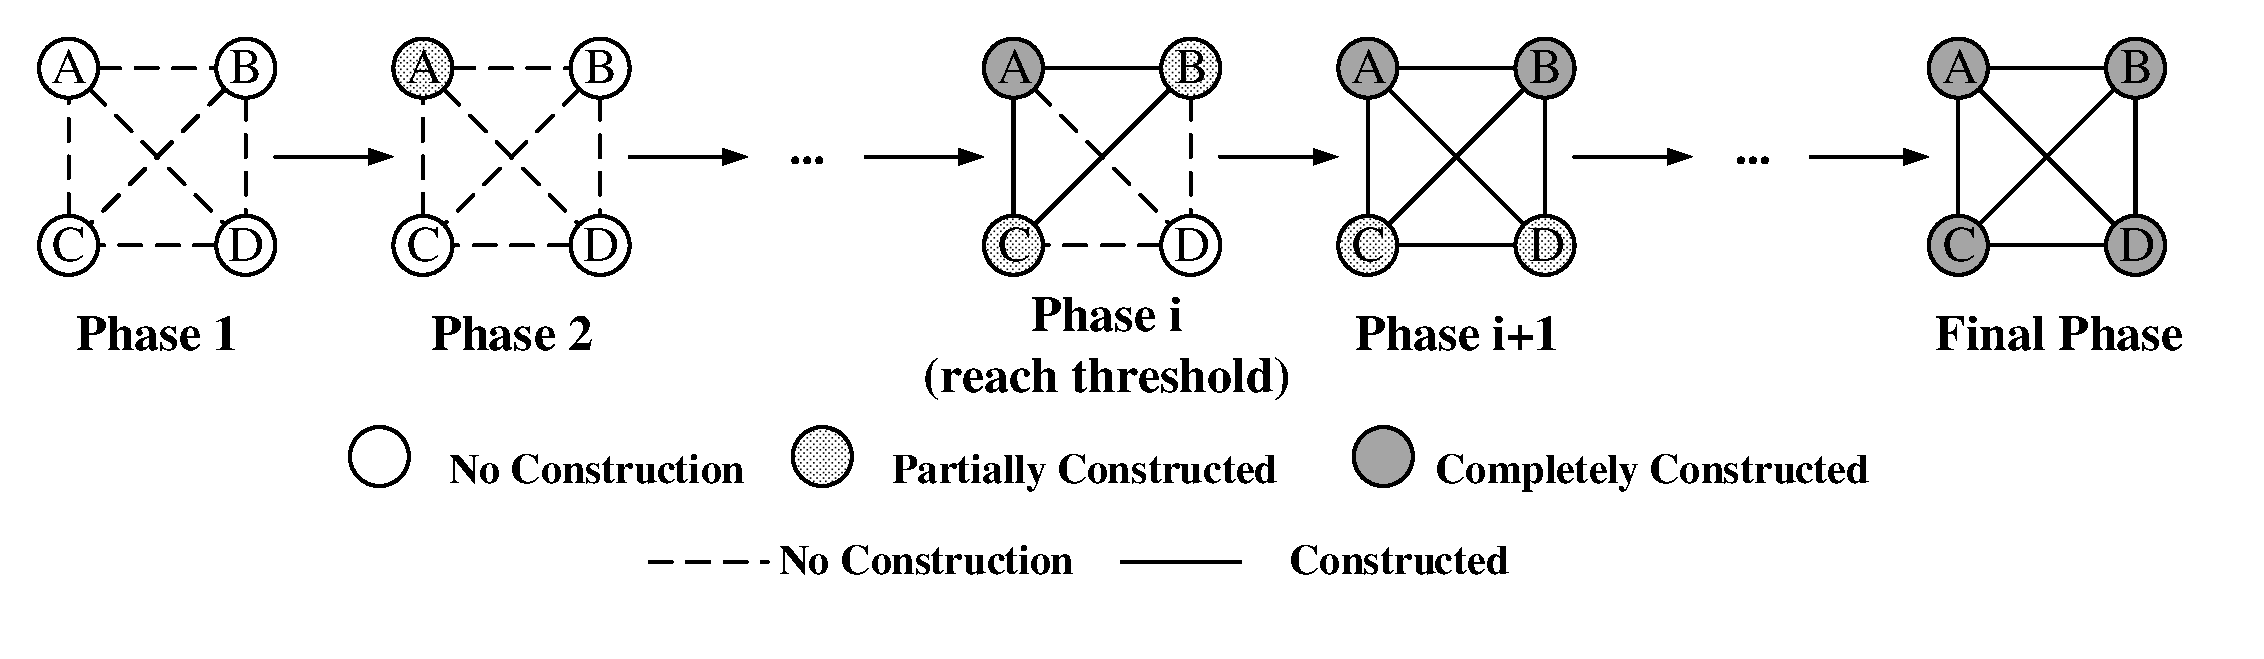
\includegraphics[width=0.99\textwidth]{Iteration.pdf}
  \caption{Process of Iterative Evolution}\label{Fig-Iteration}
\end{figure}

In this model, the process of charging network evolution is controlled by threshold $n_{ev}^{thre}$. The higher the threshold is, the slower this process will be. If the number of iterations is too large, we can decrease this threshold to accelerate the evolving process.
\subsection{Solution: Charging Network for South Korea}
To determine the final charging network under an instantaneous migration to all-electric vehicles, we just need to apply Charging Station Location Model (CSLM) to South Korea. Totally 770 charging stations need to be constructed, whose distribution is shown in Fig.~\ref{Fig-KoreaDistribution}.

\begin{figure}[htbp]
  \centering
  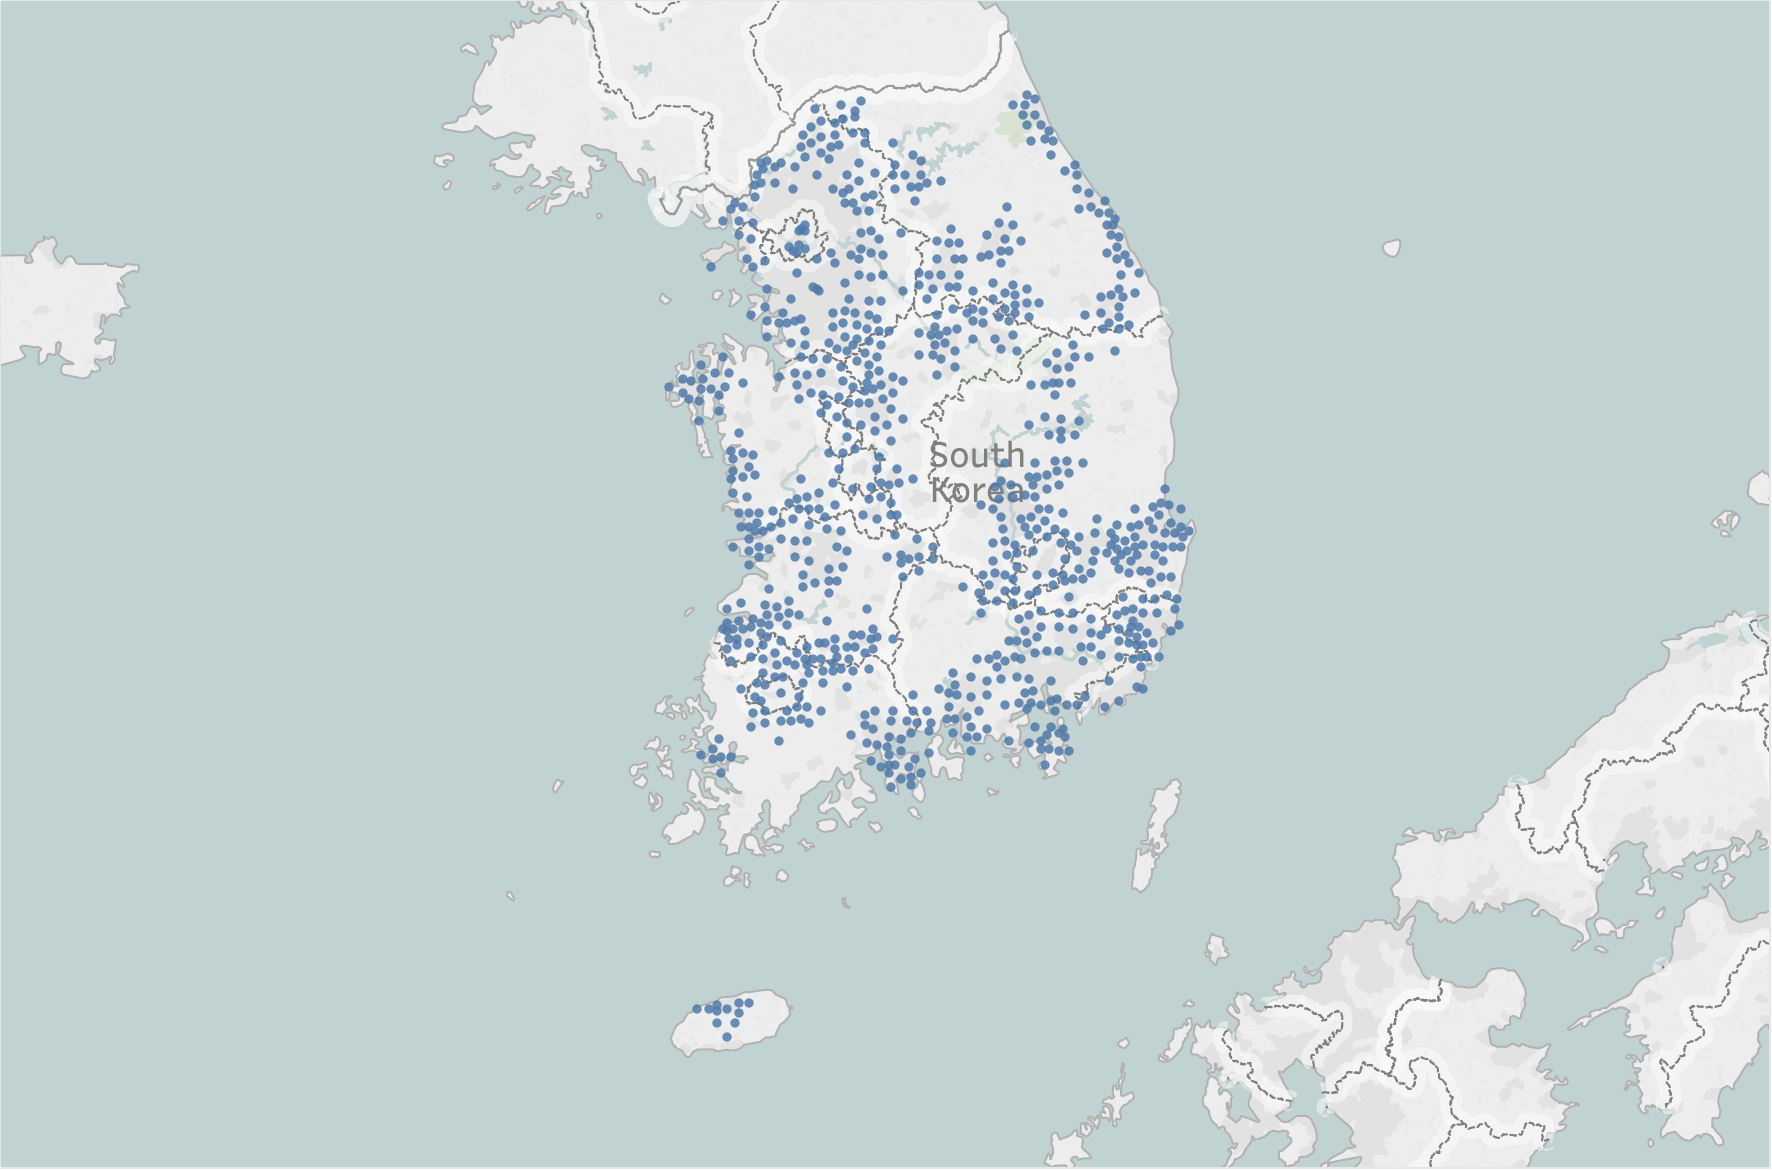
\includegraphics[width=0.6\textwidth]{KoreaDistribution.png}
  \caption{Distribution of Charging Stations in Korea}\label{Fig-KoreaDistribution}
\end{figure}

Then we apply Iterative Evolution Model for Charging Network to South Korea to determine the process of evolution. Fig.~\ref{Fig-KoreaEvolution} shows the evolving process of EV density and charging station density.

\begin{figure}[htbp]
  \centering
  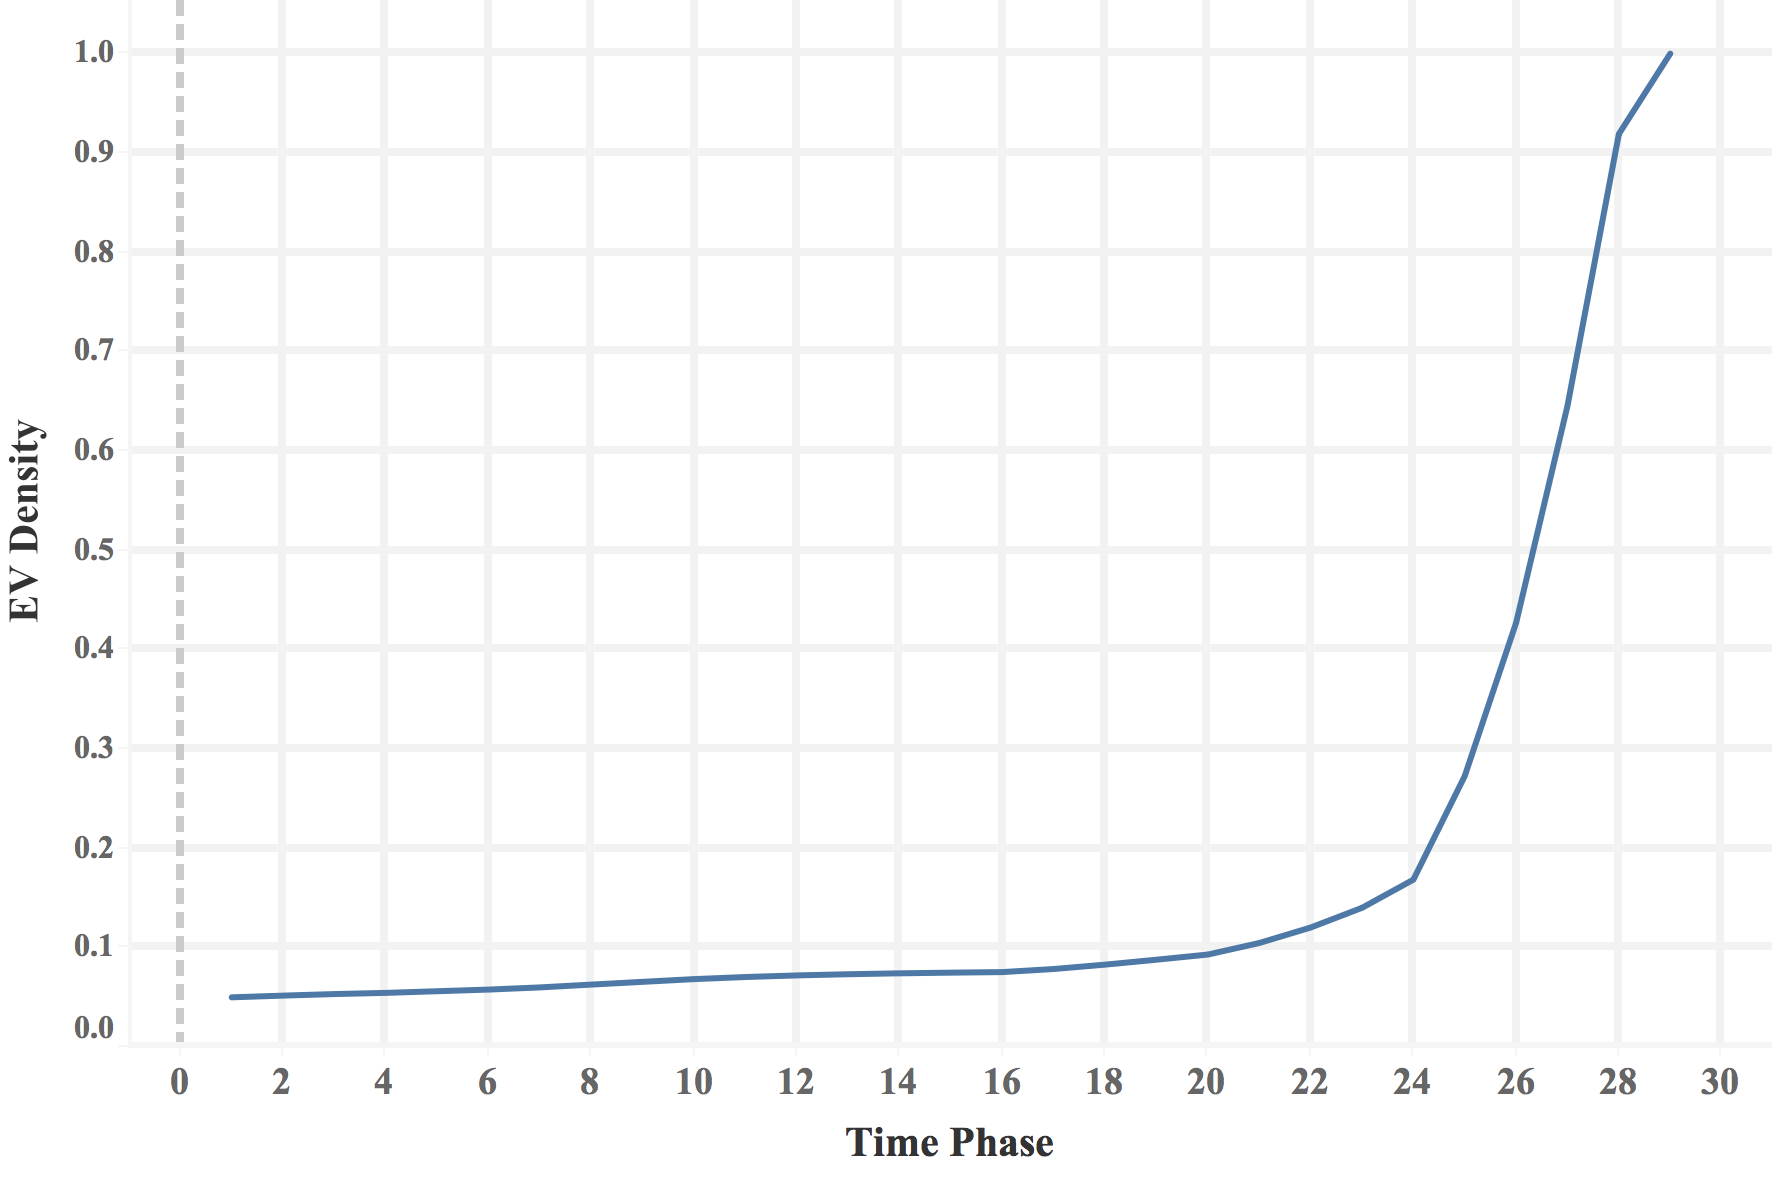
\includegraphics[width=0.6\textwidth]{KoreaEvolution.png}
  \caption{EV Density of Each Time Phase in Korea}\label{Fig-KoreaEvolution}
\end{figure}

According to our evolution model, city-based charging stations are constructed first, and then construction in both city areas and rural areas are carried out simultaneously. Since deployment of charging stations and purchase of EVs promote each other mutually, construction of charging stations should keep pace with the number of EVs.
\section{Task 3: Classification Model (CM)}\label{Sec-Task3}
\subsection{Classification Criteria and Impacts}
In this model, we set seven criteria for classifying different countries. Their impacts on our model are explained as follows.

\paragraph{Policy}
National policy for or against electric vehicles has an impact on the budget of charging network evolution. For example, China is pushing its EV development and making preparations for banning gasoline and diesel cars~\cite{ChinaBan}. There is no doubt that China will allocate a high budget to evolving charging network.

\paragraph{Wealth Distribution}
Wealth Distribution has an impact on the budget of charging network evolution and traffic flow. The transition from gasoline and diesel cars to electric cars costs a lot. In wealthier areas, a higher budget can be allocated. For example, cities in Eastern China are better developed than cities in Western China, so they can devote more money to evolving charging network. Moreover, in wealthier areas, traffic flow is usually larger. An example is still Eastern and Western China.

\paragraph{Population Distribution}
Population Distribution has an impact on traffic flow. The higher population density is, the higher traffic flow is. For example, most population in Australia is distributed in south-east coastal areas. Therefore, traffic flow in this area is much higher than in other areas.

\paragraph{Geography}
Geography has an impact on the electricity consumed for a unit distance and traffic flow. Electric vehicles consume more electricity in areas with rugged geography. For example, in Saudi Arabia where plateau covers most of its territory, EVs will consume more electricity than in plain areas for the same distance. Additionally, in areas with rugged geography, the traffic flow is usually small. Some special geographies also have an influence. For example, Indonesia is the largest archipelagic country and transportation between islands is mostly finished by air or water. In this case, the demand for charging stations along long-distance highways is relatively low.

\paragraph{Road Quality}
Road quality also has an impact on the electricity consumed for a unit distance. When road quality is poor, EVs will consume more electricity for the same distance. For example, most roads in China are constructed with high quality, while in Indonesia, roads are not so well-constructed.

\paragraph{Traffic Condition}
Traffic condition has an impact on the electricity consumed for a unit distance. Electric vehicles consume less electricity when it is travelling in a stationary manner, while sharp changes in speed results in much more electricity consumed. In countries where traffic congestion is serious, such as Indonesia and China, frequent speedup and braking cannot be avoided. Therefore, the average electricity consumed for a unit distance is higher. In countries with much sparsely populated area, it is lower.

\paragraph{Territory Area}
Territory area has an impact on the necessity of applying Interstate CSLM in Section~\ref{Sec-Interstate}. For countries with huge territory, such as China and Australia, a large number of highways crisscross the land connecting different parts of the country. In these countries, constructing charging stations along interstate highways is of great significance. However, in countries such as Singapore, there is no need to apply Interstate CSLM due to its small territory area.


For clarity, all the criteria and their impacts are listed in Table~\ref{Tlb-ClassificationCriteria}. If a criterion has an impact, there is a tick in the corresponding cell.

\begin{table}[htbp]
  \centering
  \caption{Classification Criteria and Impacts}\label{Tlb-ClassificationCriteria}
  \begin{tabular}{ccccc}
    \hline
      & Budget & Traffic Flow & Electricity & Interstate CSLM \\
    \hline
    Policy & \checkmark &   &   &   \\
    Wealth Dist. & \checkmark & \checkmark &   &   \\
    Population Dist. &   & \checkmark &   &   \\
    Geography &   & \checkmark & \checkmark &   \\
    Road Quality &   &   & \checkmark &   \\
    Traffic Condition &   &   & \checkmark &   \\
    Territory Area &   &   &   & \checkmark \\
    \hline
  \end{tabular}
\end{table}
\subsection{Modification}
Based on the analysis above, our model for evolving charging network do not apply to some countries due to specific reasons. However, in the following, we show that our model can be adapted to many different countries only by a slight modification.

\paragraph{Policy}
The threshold for the number of EVs in a city $n_{ev}^{thre}$ in Section~\ref{Sec-IEMEstablishment} is related to budget. The higher the budget is, the lower this threshold is. Therefore, we add a coefficient to $n_{ev}^{thre}$ and have a new threshold $\gamma_{policy}n_{ev}^{thre}$. For countries supporting electric vehicle development, $\gamma_{policy}$ is smaller than 1. If countries against electric vehicles, $\gamma_{policy}$ is larger than 1.

\paragraph{Wealth Distribution}
In terms of budget, same as policy, we add a coefficient to $n_{ev}^{thre}$ and have a new threshold $\gamma_{policy}\gamma_{wealth}n_{ev}^{thre}$. For wealthy areas, $\gamma_{wealth}$ is larger than 1. For poorly developed areas, $\gamma_{wealth}$ is smaller than 1. In terms of traffic flow, origin-destination pairs (O-D pairs) generated in Interstate CSLM should be considered. In Section~\ref{Sec-Interstate}, O-D pairs are randomly generated, and thus uniformly distributed across the whole country. However, traffic flow may not be evenly distributed. Therefore, we skew the generation of O-D pairs in favour of areas with higher traffic flow.

\paragraph{Population Distribution}
Same as wealth distribution, we skew the generation of O-D pairs in favour of areas with higher population density.

\paragraph{Geography}
In terms of electricity consumed for a unit distance, we add a coefficient to $w$, which is the electricity consumed for a unit distance in Eqn.~\eqref{Eqn-StateOfCharge}. We have $\gamma_{geography}w$, where $\gamma_{geography}$ is larger than 1 in rugged areas and $\gamma_{geography}$ is smaller than 1 in plain areas. For countries with specific geography characteristics, we should modify our model correspondingly.

\paragraph{Road Quality}
Same as geography, we add a coefficient to $w$ and get a new consumption for a unit distance $\gamma_{geography}\gamma_{road}w$. For countries with high road quality, $\gamma_{road}$ is smaller than 1. For countries with poor road quality, $\gamma_{road}$ is larger than 1.

\paragraph{Traffic Condition}
Same as geography, we add a coefficient to $w$ and get a new consumption for a unit distance $\gamma_{geography}\gamma_{road}\gamma_{traffic}w$. For countries with serious traffic congestion, $\gamma_{road}$ is larger than 1. For countries with smooth traffic, $\gamma_{road}$ is smaller than 1.

\paragraph{Territory Area}
For countries with small territory area, we may considering ignoring Interstate CSLM but just focusing on Intrastate CSLM.
\section{Task 4: Impacts of Emerging Technologies on Charging Network Evolution}\label{Sec-Task4}
In this section, we discuss how the new transportation options impact on the evolution of charging network. Impacts are mainly divided into two types: impact on the number of electric vehicles and the deployment of charging stations. Note that those impact one of them also have an indirect impact on the other.
\subsection{Impact on the Number of EV}
\subsubsection*{Self-Driving Cars}
Most self-driving cars will be electric vehicles. The reason for this is that EVs are environment-friendly and they are easy to control by computers. \cite{SelfDriving} proposes that ``the future of autonomous vehicles is directly tied to the cost-effectiveness of electric vehicles'', which means the demand for EVs will rise sharply with the development of self-driving cars. Therefore, the advance of self-driving technology will result in increasing number of EVs.
\subsubsection*{Hyperloop}
``Hyperloop is an entirely new, disruptive, and somewhat provocative, travel mode proposition based on the use of sealed tube systems through which pods could travel free of air resistance with speeds exceeding 1000 km/h''~\cite{Nikitas2017}. As a completely different travel mode, Hyperloop achieves better transportation performance than electric vehicles and can be an alternative to EV. \cite{Nikitas2017} proposes that it is widely agreed that Hyperloop will take the place of current mobility service rather than complementing it. Based on this idea, we think most long-distance trips will be realized by Hyperloop while daily business trips will still be realized by EVs. Therefore, Hyperloop will result in only a slight decline in the number of EVs and destination charging stations but a sharp decline in the number of supercharging stations.
\subsection{Impact on the Deployment of Charging Stations}
\subsubsection*{Car-Share and Ride-Share Services}
\cite{SharedEV} puts forward the following opinion. Shared EVs only make profit when carrying customers around, and charging time is downtime for shared EVs. For a shared EV, it cannot be tolerated to spend many hours having it charged. The ideal case for a shared EV is that it can get charged quickly wherever it is, which requires high availability of charging stations. Therefore, the development of car-share and ride-share services will result in increasing number of charging stations.
\subsubsection*{Rapid Battery-Swap Stations for Electric Cars}
Battery-swap station is an alternative to traditional destination charging station and supercharging station. Its advantage is the high efficiency of charging, while the cost of it is quite high. Therefore, battery-swap stations may take the place of parts of traditional charging stations, since some people want rapid charging for their EVs to save time. However, not all the traditional charging stations will be replaced due to the high cost of charging.
\subsubsection*{Flying Cars}
In \cite{FlyingCar}, it is mentioned that Uber adds ultra-super chargers to the existing charging stations to satisfy the charging need of flying cars. Inspired by this, we think a new kind of charger specifically designed for flying cars will be constructed, mainly in existing stations to save cost. However, the distribution of this new kind of charger does not follow the traditional traffic network, but is determined by a specific network of flying cars.
\section{Model Analysis}\label{Sec-Analysis}
\subsection{Sensitivity Analysis}
Determining the timeline for evolving charging network is of great significance. However, in Iterative Evolution Model for Charging Network, there is much uncertainty concerning two parameters: $n_{ev}^{thre}$ and $den_{ev}^{(1)}$. Value of $n_{ev}^{thre}$ changes under many circumstances. For example, if a country faces financial deficit, there will not be enough budget for constructing charging stations. $den_{ev}^{(1)}$ indicates the interest of consumers in EV when they first enter the market, which is hard to estimate precisely. Therefore, there is necessity that we examine the stability of our model.

Firstly, we fix $n_{ev}^{thre}$ and check how the result changes as $den_{ev}^{(1)}$ fluctuates. The results are shown in Fig.~\ref{Fig-SenDen}.

\begin{figure}[htbp]
    \centering
    \begin{subfigure}[b]{0.45\textwidth}
		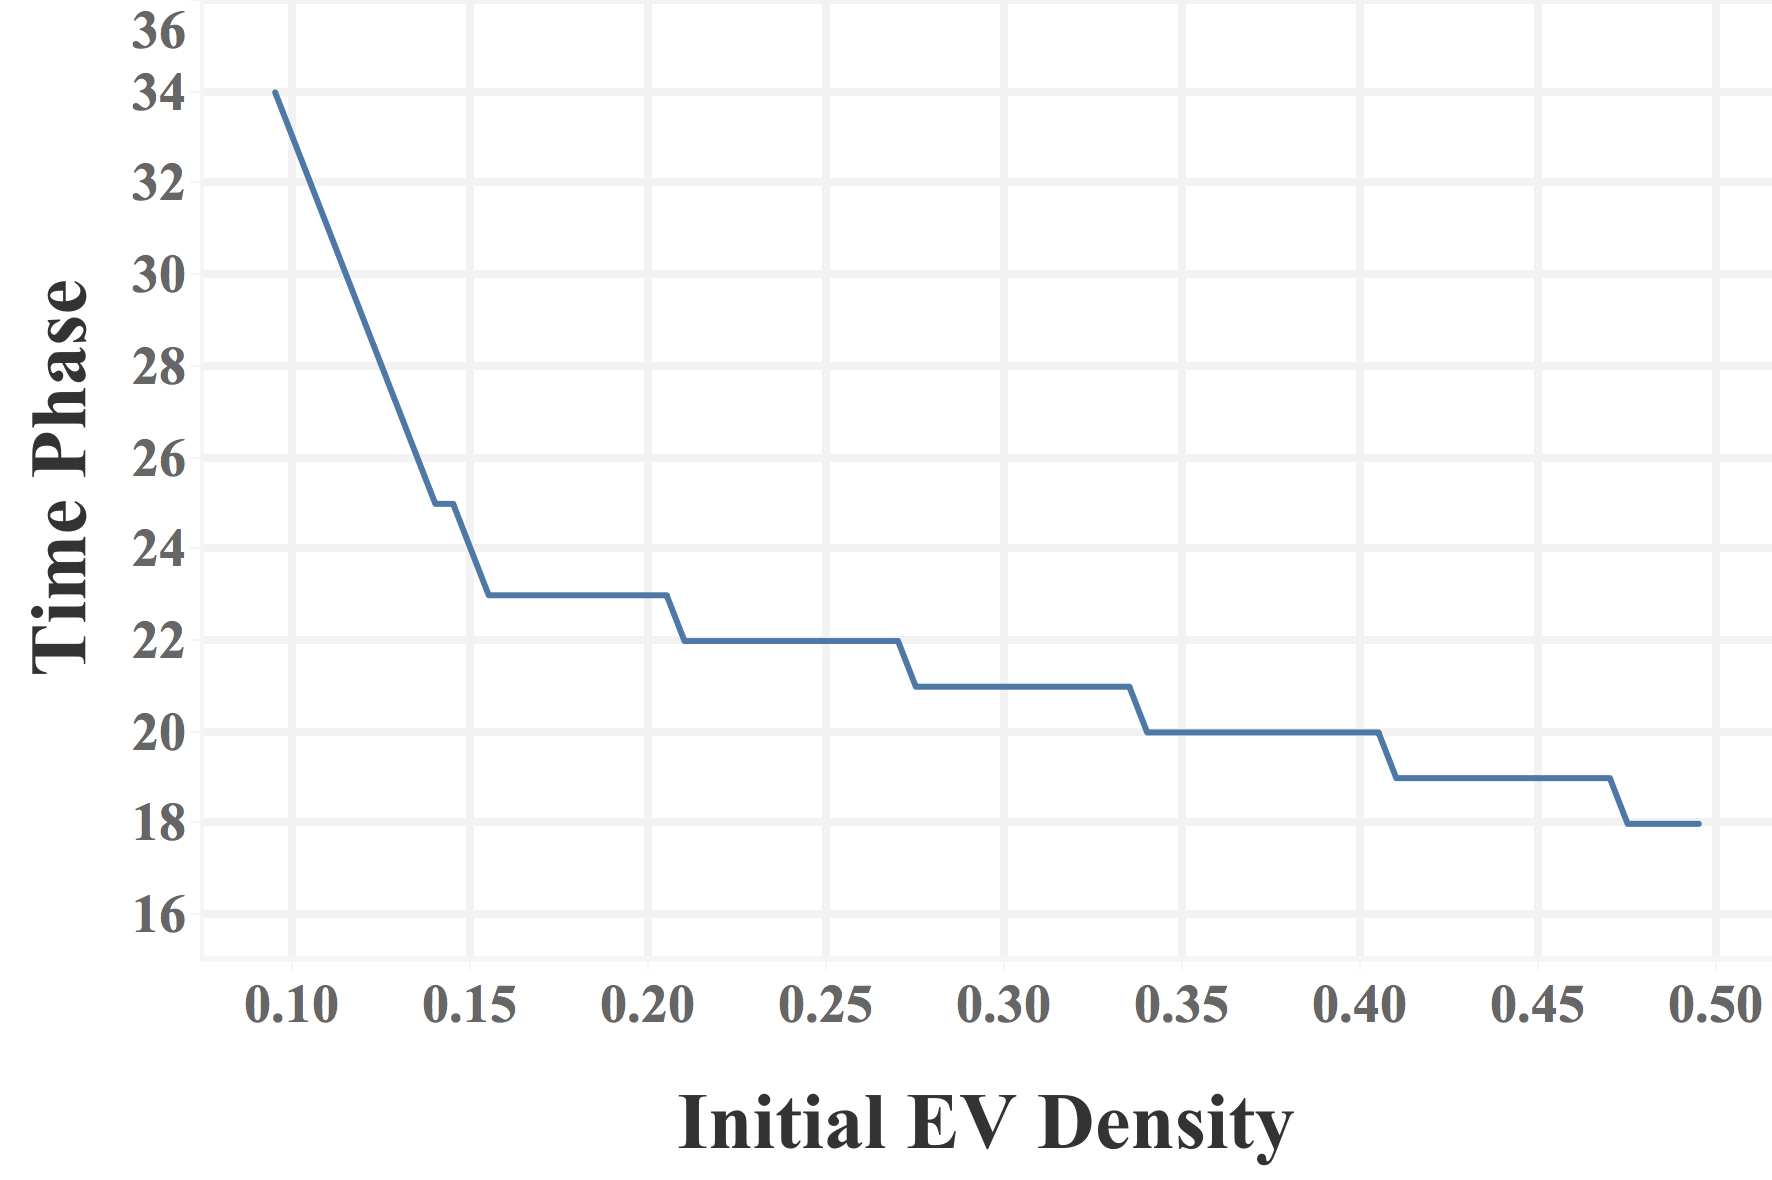
\includegraphics[width=0.95\textwidth]{PhaseDen.png}
	\end{subfigure}
    \begin{subfigure}[b]{0.45\textwidth}
		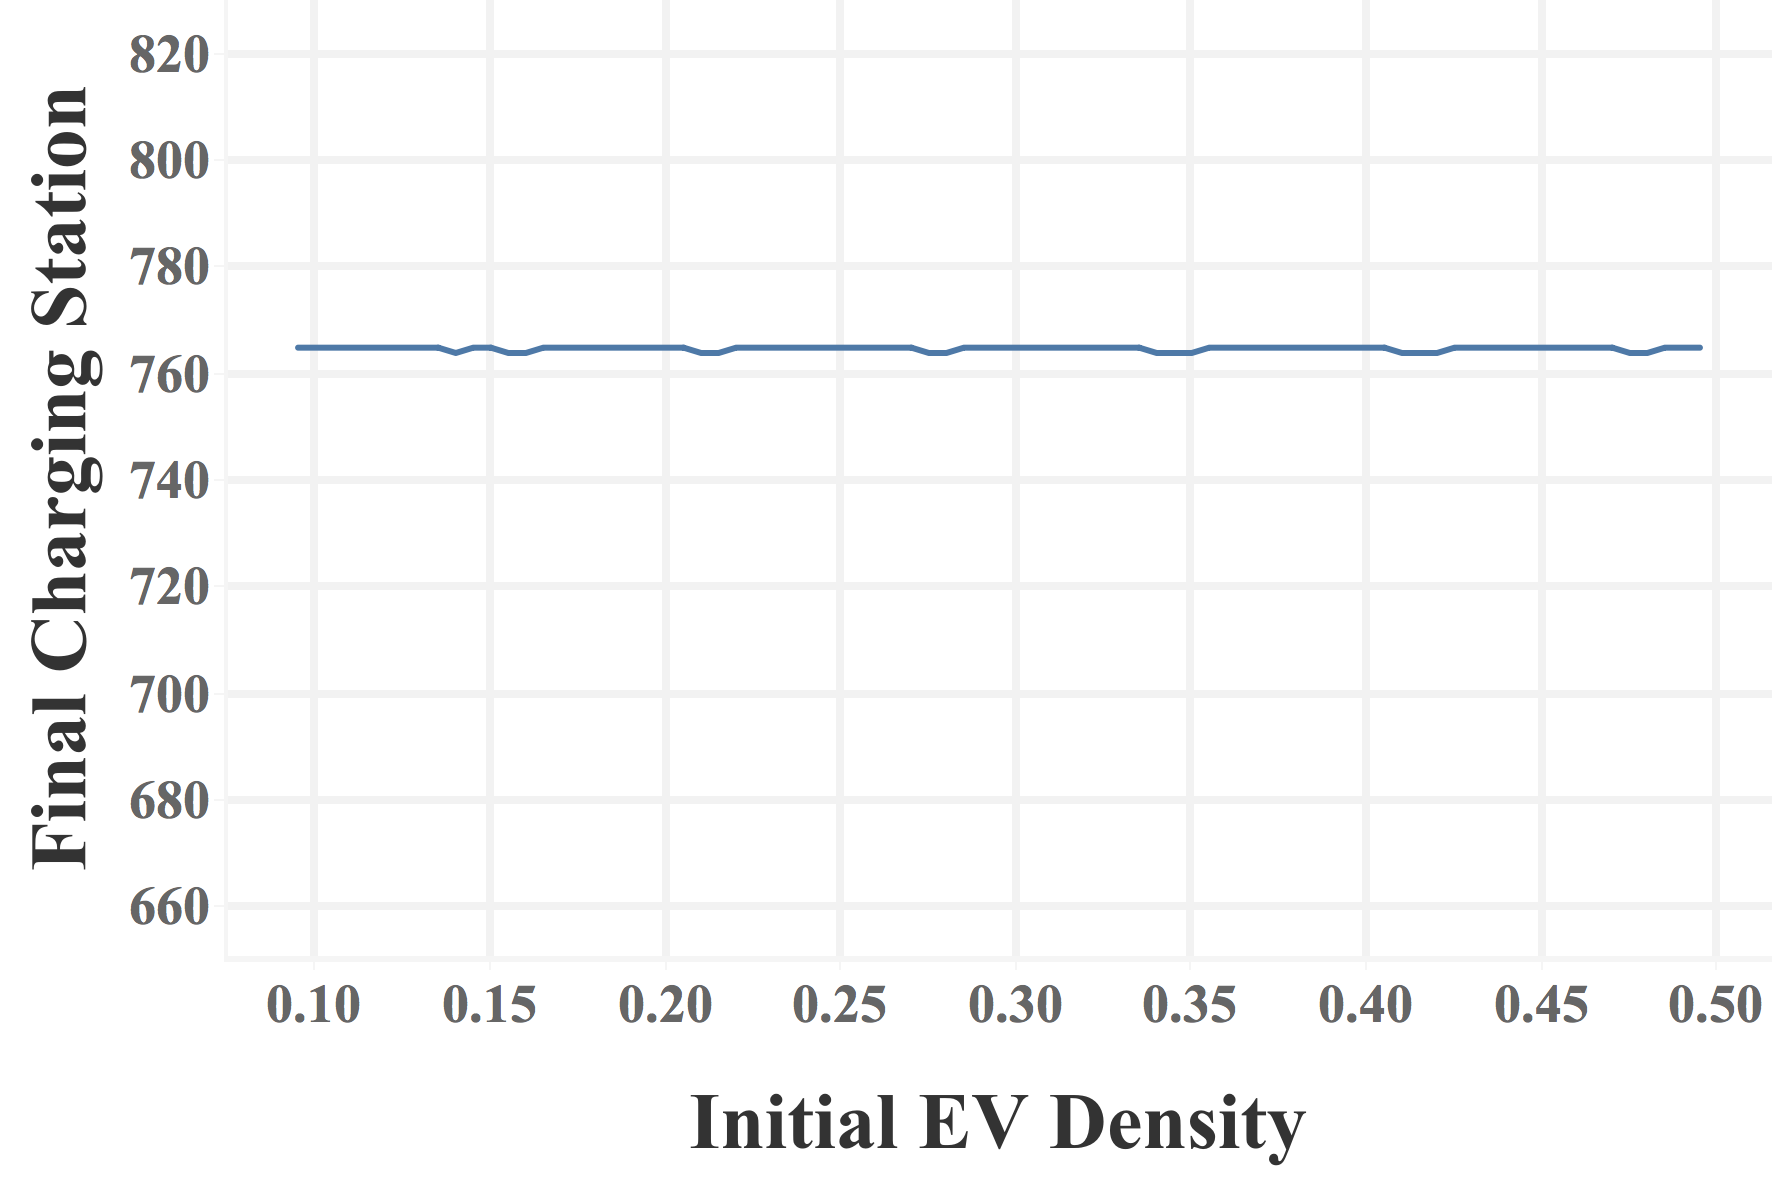
\includegraphics[width=0.95\textwidth]{ChargerDen.png}
	\end{subfigure}
    \caption{Sensitivity Analysis of $den_{ev}^{(1)}$}\label{Fig-SenDen}
\end{figure}
From Fig.~\ref{Fig-SenDen}, we can conclude that value of $den_{ev}^{(1)}$ has little impact on the number of phases, while it has a great impact on final number of charging stations.

Secondly, we fix $den_{ev}^{(1)}$ and check how the result changes as $n_{ev}^{thre}$ fluctuates. The results are shown in Fig.~\ref{Fig-SenThre}.

\begin{figure}[htbp]
    \centering
    \begin{subfigure}[b]{0.45\textwidth}
		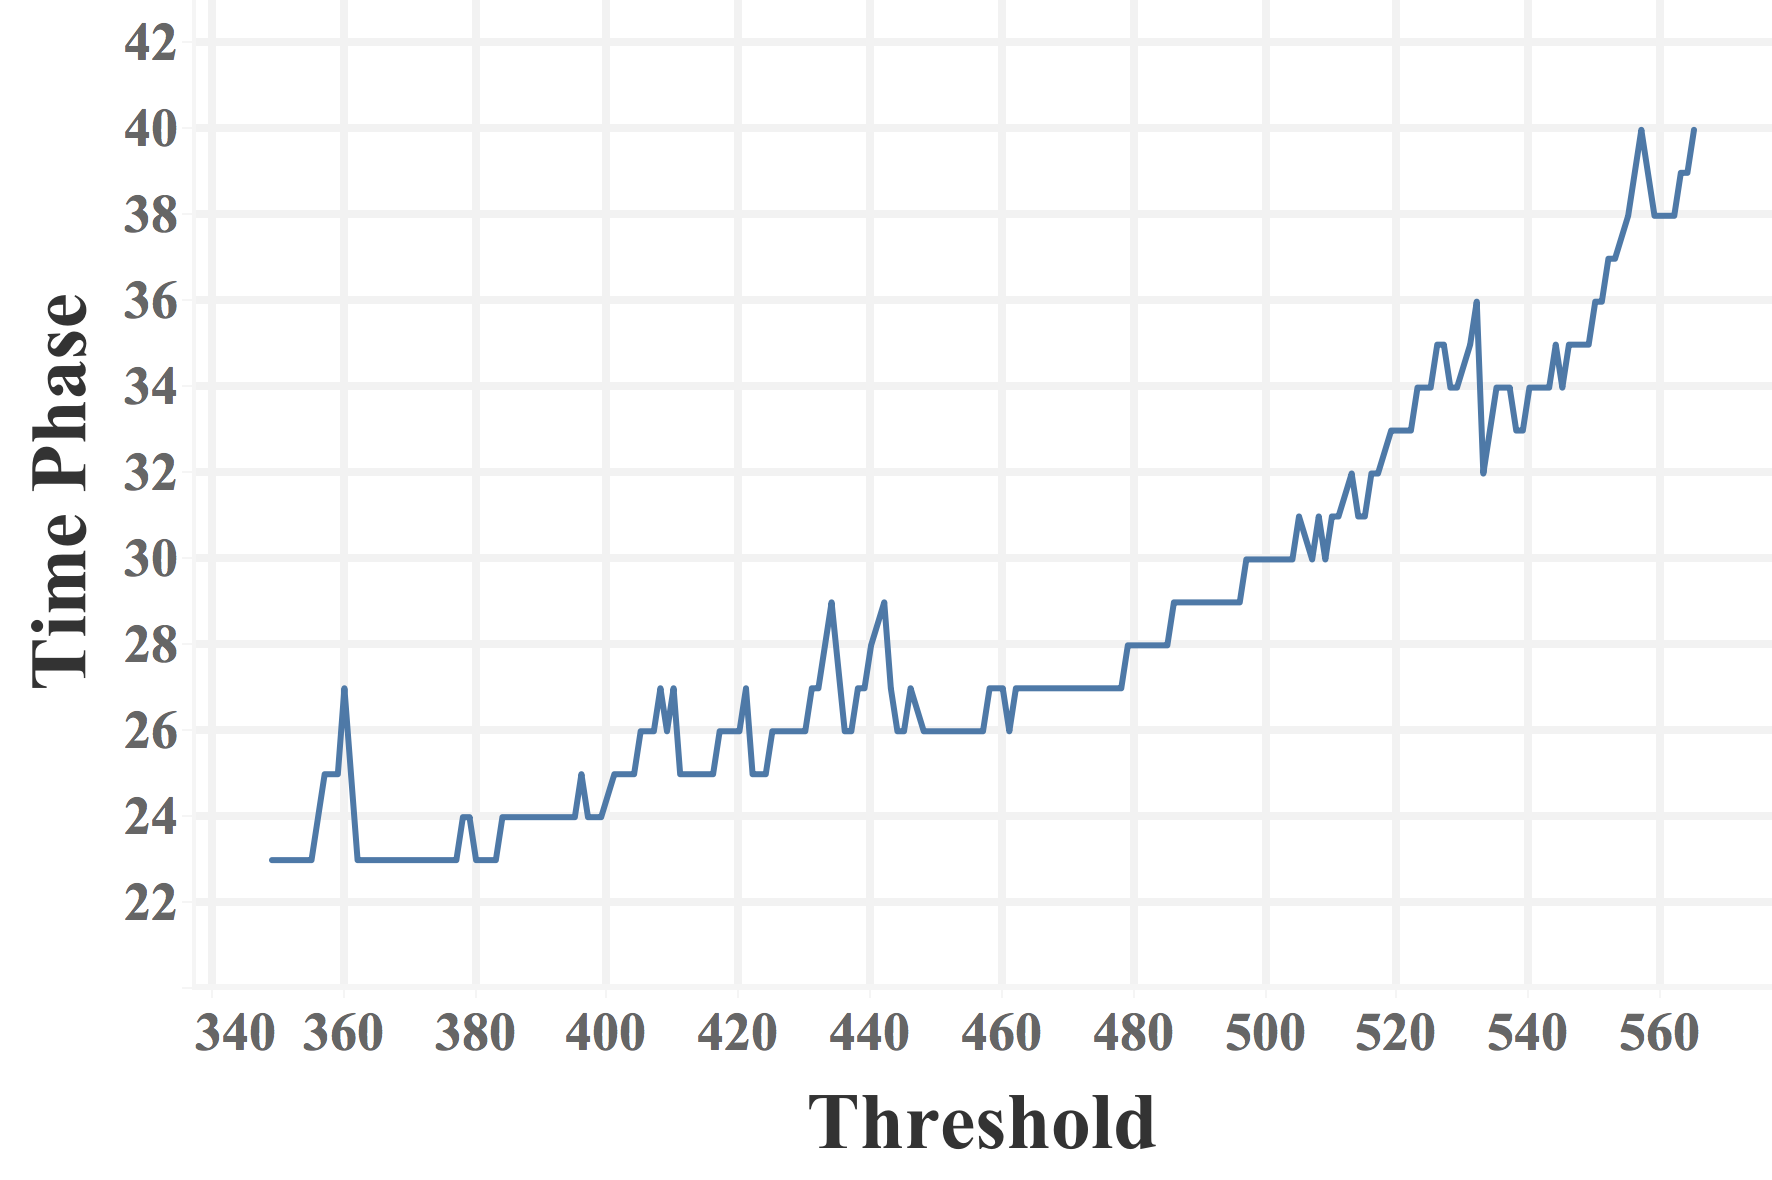
\includegraphics[width=0.95\textwidth]{PhaseThre.png}
	\end{subfigure}
    \begin{subfigure}[b]{0.45\textwidth}
		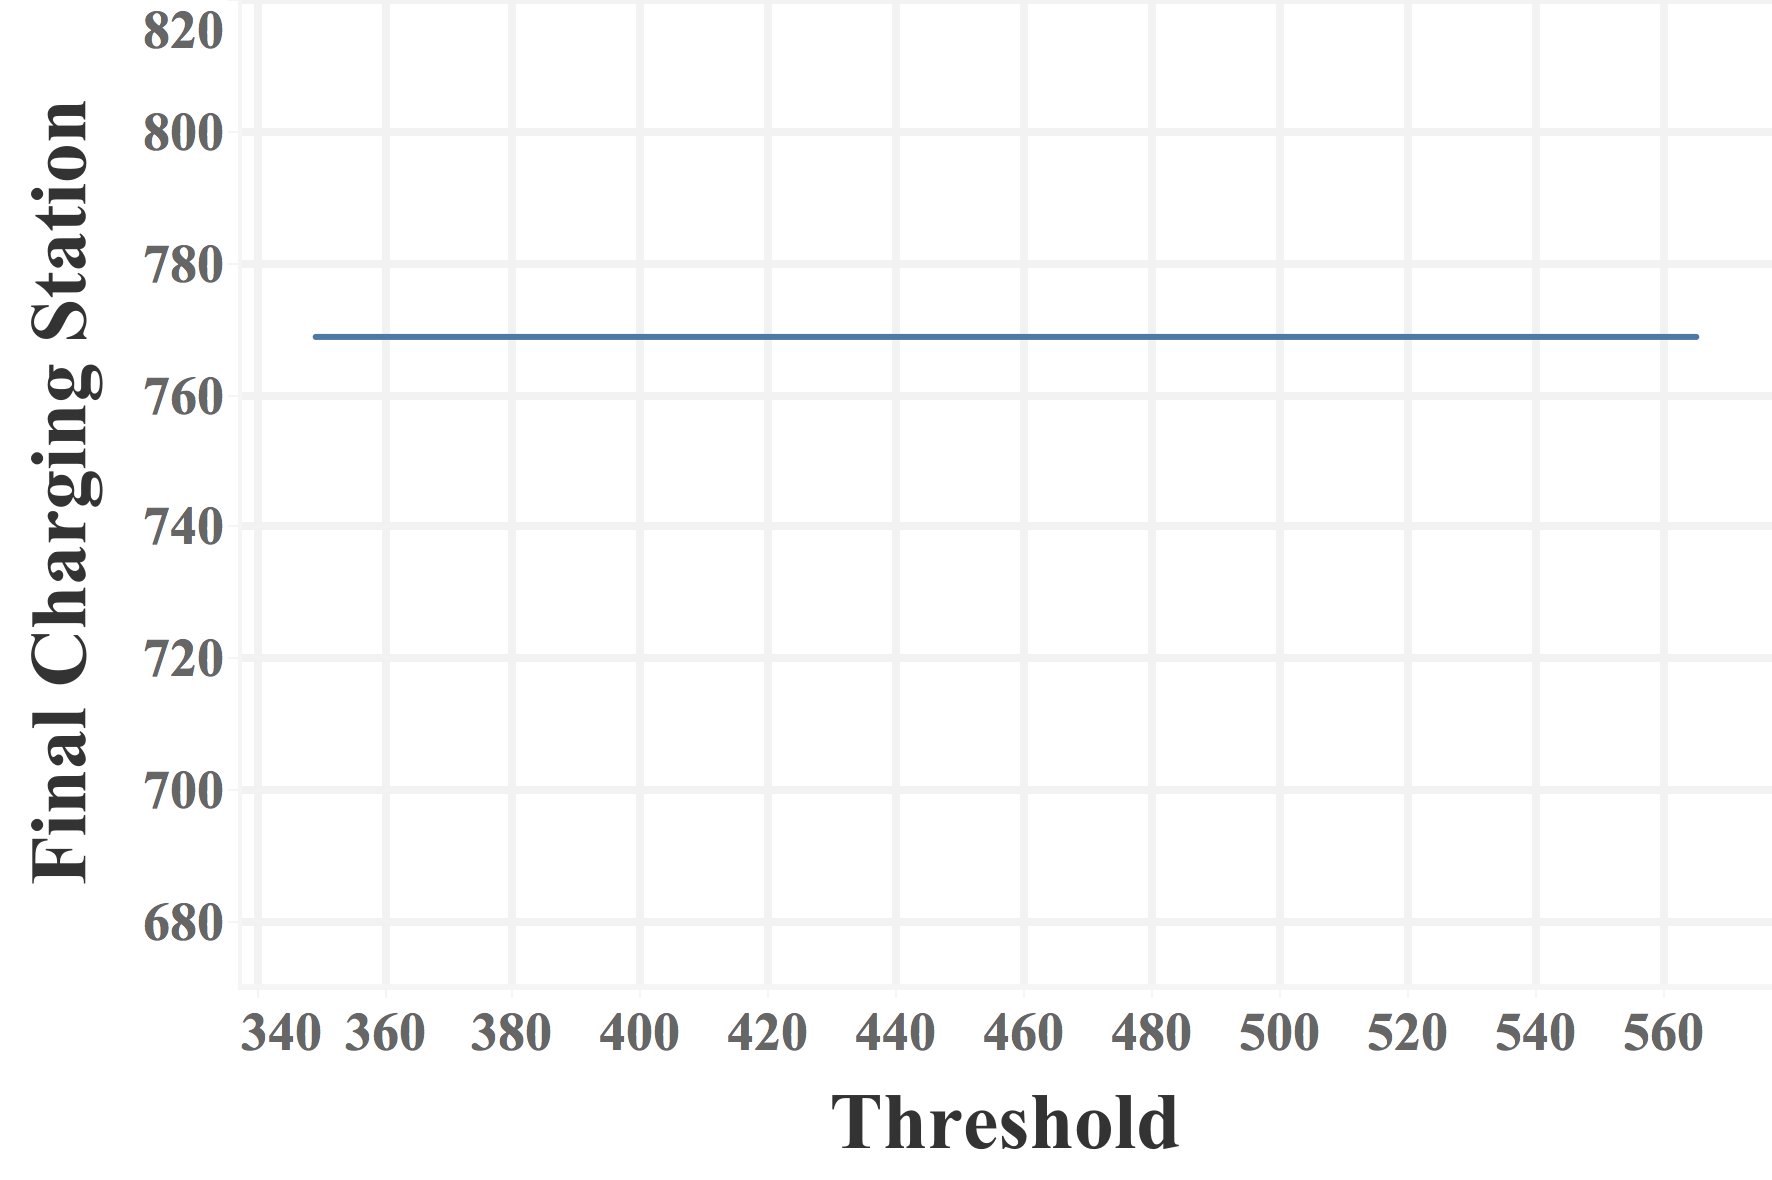
\includegraphics[width=0.95\textwidth]{ChargerThre.png}
	\end{subfigure}
    \caption{Sensitivity Analysis of $den_{ev}^{(1)}$}\label{Fig-SenThre}
\end{figure}
From Fig.~\ref{Fig-SenThre}, we can conclude that value of $n_{ev}^{thre}$ has little impact on final number of charging stations, while it has a great impact on the number of phases.
\subsection{Strengths and Weaknesses}
\subsubsection*{Strengths}
\begin{enumerate}
\item We adopt the professional concept of traffic analysis zone (TAZ) in Charging Station Location Model. TAZ can describe traffic activity of a particular region, which gives us accurate information about the distribution of demand for charging stations.
\item We make a complementary combination between node-covering model and flow-capturing model, and thus build targeted models for intrastate and interstate conditions.
\item Due to a lack of road information, we make full use of accessible facts by combining simulation with clustering in Interstate CSLM, which uses charging point to illustrate the road information.
\item Based on the fact that deployment of charging stations and purchase of EV promote each other, we use iteration model to determine a detailed timeline for evolving charging network.
\end{enumerate}
\subsubsection*{Weaknesses}
\begin{enumerate}
\item Our Charging Station Location Model can only determine the construction of one type of chargers, which means the demand for supercharging stations is ignored in daily business areas.
\item In Iterative Evolution Model for Charging Network, the duration between two time phases is defined subjectively, which may not be the optimal. Determination of it needs further discussion.
\end{enumerate}
\subsection{Personal to Commercial}
For commercial cars, especially heavy trucks and buses, since the distance they travel is usually very long, their demand for supercharging stations is higher than for destination charging stations. According to this, construction of supercharging stations along highways should pay special attention to these types of vehicles.

Moreover, heavy trucks and buses consumes more electricity, while their downtime for charging is short. As a result, charging stations should stay idle for them, and even a new type of charger should be designed to meet the charging demand of them.
\section{Conclusion} \label{Sec-Conclusion}
In this paper, we propose CNEM, which is composed of Charging Station Location Model (CSLM), Iterative Evolution Model for Charging Network (CN-IEM), and Classification Model (CM). CSLM takes advantage of node-covering model and flow-capturing model and uses Fuzzy C-Means (FCM) clustering algorithm to obtain better location selection. CN-IEM considers the mutual promotion of the deployment of charging stations and the purchase of EV and adopts iterative evolution model to simulate their interaction over time. In CM, we set seven classification criteria and present corresponding modification to adapt our model to different countries. We explain how emerging technologies impact on the charging network. We also make sensitivity analysis and present the strength and weakness of our models. Experiments of CSLM and CN-IEM are conducted for United States and South Korea respectively. Results prove the effectiveness of our models.

\newpage
\section*{Handout for Nation Leadership}
\addcontentsline{toc}{section}{Handout for Country Leadership}
\noindent To nation leadership:

\smallskip

To construct a full-electric charging network in your country, here is a list of things worth considering.

\begin{itemize}
\item Investigate several indexes in your country first.

Major indexes include policy towards EV, wealth distribution, population distribution, geography, road quality, traffic condition, and territory area.

These indexes indicate conditions for building a full-electric charging network, and can help construct a more customized network for your country.
\item Draw the blueprint

Based on the indexes, Interstate and Intrastate Location Model are carried out. The former is used to meet the charging demand within a state (or province), and the latter is applied to capture the demand on nationwide highway system. Furthermore, two types of chargers with different power are distributed accordingly considering the resource allocation between daily business and long-distance trip. Therefore, these models can be applied to draw the blueprint of the final status of the full-electric charging network, which can be seen as a guidance for its evolution.
\item Determine the evolution timeline

On the basis of the blueprint, given the indexes of your country, a customized evolution model can be used to determine the schedule of evolving the charging network. The model can provide precise information including the exact number, location, distribution of new charging stations in each time phase. That is to say, it presents a timeline for evolution from which the nation can foresee what is supposed to happen before the fully construction of charging network.
\item Influential factors

New emerging technologies may influence the construction of charging network. Positive factors, such as the development of car-sharing services, will expand the demand for charging stations. Negative factors, such as rapid battery-swap station, will reduce the demand for charging stations. Controlling the impact of new technologies on the number of electric vehicles and demand for charging stations is a key factor of the construction speed of charging network.
\end{itemize}

Although the process of building a charging network may be long and sometimes worrisome, it is the basic to a prosperous future with clean energy.

For further information, please refer to our paper.

\smallskip

\noindent Team \#72985

\newpage

\bibliographystyle{unsrt}
\bibliography{bibfile}
	
%\newpage
%\section*{Executive Summary}
	
%\noindent To whom it may concern,
	
\end{document}

%%
%% This work consists of these files mcmthesis.dtx,
%%                                   figures/ and
%%                                   code/,
%% and the derived files             mcmthesis.cls,
%%                                   mcmthesis-demo.tex,
%%                                   README,
%%                                   LICENSE,
%%                                   mcmthesis.pdf and
%%                                   mcmthesis-demo.pdf.
%%
%% End of file `mcmthesis-demo.tex'.
